\documentclass[12pt]{article}
%\usepackage{natbib}
\usepackage[numbers]{natbib}
\usepackage{amsthm}
\usepackage[toc,page]{appendix}
\usepackage{color}
\usepackage{graphicx}
\usepackage{tabularx}
\usepackage{caption}

\usepackage{longtable}
\usepackage[]{inputenc}
\usepackage[T1]{fontenc}
\usepackage{fullpage}
\usepackage{coqdoc}
\usepackage{amsmath,amssymb}
\usepackage{listings}


\DeclareGraphicsExtensions{.pdf,.png,.jpg}
\definecolor{codegreen}{rgb}{0,0.6,0}
\definecolor{codegray}{rgb}{0.5,0.5,0.5}
\definecolor{codepurple}{rgb}{0.58,0,0.82}
\definecolor{backcolour}{rgb}{0.95,0.95,0.92}

\DeclareCaptionFormat{listing}{#1#2#3}
\captionsetup[lstlisting]{format=listing,singlelinecheck=false} 

\lstdefinestyle{mystyle}{
    backgroundcolor=\color{backcolour},   
    commentstyle=\color{codegreen},
    keywordstyle=\color{magenta},
    numberstyle=\tiny\color{codegray},
    stringstyle=\color{codepurple},
    basicstyle=\footnotesize,
    breakatwhitespace=false,         
    breaklines=true,                 
    captionpos=b,                    
    keepspaces=true,                 
    numbers=left,                    
    numbersep=5pt,                  
    showspaces=false,                
    showstringspaces=false,
    showtabs=false,                  
    tabsize=2
}
\newtheorem{mydef}{Definition}


\begin{document}

\begin{appendices}
\end{appendices}
\section{Full Results - Other Languages}
\label{FullResultsOther}
\subsection{Table - DFA2 Analysis results per source file}
TODO cite these
\begin{longtable}{l l r r r}
\textbf{Filename} & \textbf{Type} & \textbf{H} & \textbf{+/-} & \textbf{R} \\
{jquery-1.11.1.js} & naive & 0.58557 & 0.010196 & 0.99911 \\
{jquery-1.11.1.js} & trim & 0.58759 & 0.010714 & 0.99902 \\
{message.rb} & trim & 0.5677 & 0.01124 & 0.99885 \\
{jquery-1.11.1.js} & tab3 & 0.61124 & 0.01249 & 0.99877 \\
{message.rb} & naive & 0.56266 & 0.012069 & 0.99865 \\
{message.rb} & tab3 & 0.56266 & 0.012069 & 0.99865 \\
{message.rb} & tab8 & 0.56266 & 0.012069 & 0.99865 \\
{StorageService.java} & tab8 & 0.67267 & 0.01641 & 0.99825 \\
{StorageService.java} & naive & 0.6721 & 0.016419 & 0.99825 \\
{StorageService.java} & tab3 & 0.67223 & 0.016457 & 0.99824 \\
{jquery-1.11.1.js} & tab8 & 0.72399 & 0.019735 & 0.99782 \\
{StorageService.java} & trim & 0.61487 & 0.022114 & 0.99621 \\
{BigInteger.cs} & trim & 0.70561 & 0.025801 & 0.99608 \\
{BigInteger.cs} & naive & 0.70258 & 0.028364 & 0.99523 \\
{BigInteger.cs} & tab3 & 0.70918 & 0.033326 & 0.99356 \\
{tests.py} & tab8 & 0.58898 & 0.029061 & 0.9929 \\
{tests.py} & naive & 0.58898 & 0.029061 & 0.9929 \\
{tests.py} & tab3 & 0.58898 & 0.029061 & 0.9929 \\
{tests.py} & trim & 0.63369 & 0.032319 & 0.99242 \\
{activerecord.html} & naive & 0.4035 & 0.021247 & 0.99193 \\
{activerecord.html} & tab3 & 0.4035 & 0.021247 & 0.99193 \\
{activerecord.html} & tab8 & 0.4035 & 0.021247 & 0.99193 \\
{BigInteger.cs} & tab8 & 0.74006 & 0.043006 & 0.99019 \\
{activerecord.html} & trim & 0.40015 & 0.027494 & 0.98637 \\
\end{longtable}

\newpage
\subsection{Table - DFA2 Variance - Other Languages}\label{FullResultsOtherVariance}
\begin{longtable}{l r}
\textbf{Filename} &  \textbf{H} \\
{activerecord.html} & 0.0033500000000000196  \\
{BigInteger.cs} & 0.03748000000000007  \\
{jquery-1.11.1.js} & 0.13842  \\
{message.rb} & 0.005039999999999933  \\
{StorageService.java} & 0.05779999999999996  \\
{tests.py} & 0.04471000000000003  \\
\end{longtable}
\begin{longtable}{l r}
\textbf{Filename} &  \textbf{+/-} \\
{activerecord.html} & 0.0062470000000000026  \\
{BigInteger.cs} & 0.017205  \\
{jquery-1.11.1.js} & 0.009538999999999999  \\
{message.rb} & 0.0008289999999999999  \\
{StorageService.java} & 0.005704000000000001  \\
{tests.py} & 0.0032580000000000005  \\
\end{longtable}
\begin{longtable}{l r}
\textbf{Filename} &  \textbf{R} \\
{activerecord.html} & 0.005560000000000009  \\
{BigInteger.cs} & 0.005889999999999951  \\
{jquery-1.11.1.js} & 0.0012900000000000134  \\
{message.rb} & 0.00019999999999997797  \\
{StorageService.java} & 0.0020399999999999308  \\
{tests.py} & 0.00048000000000003595  \\
\end{longtable}

\newpage
\subsection{Graphs - Other Languages}
\begin{center}
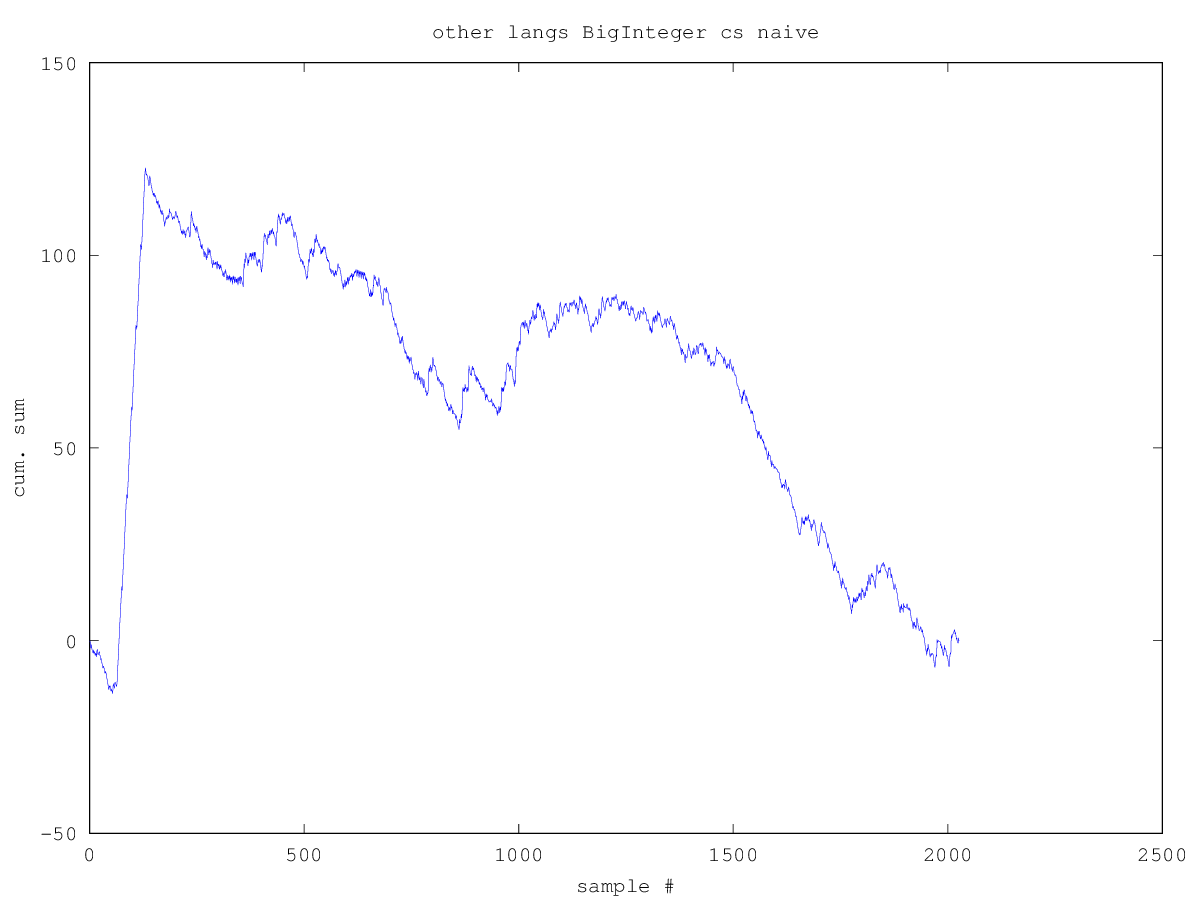
\includegraphics[width=0.8\linewidth]{{fractals/other_lang_data/other_langs_BigInteger_cs_naive_time_series}.png}
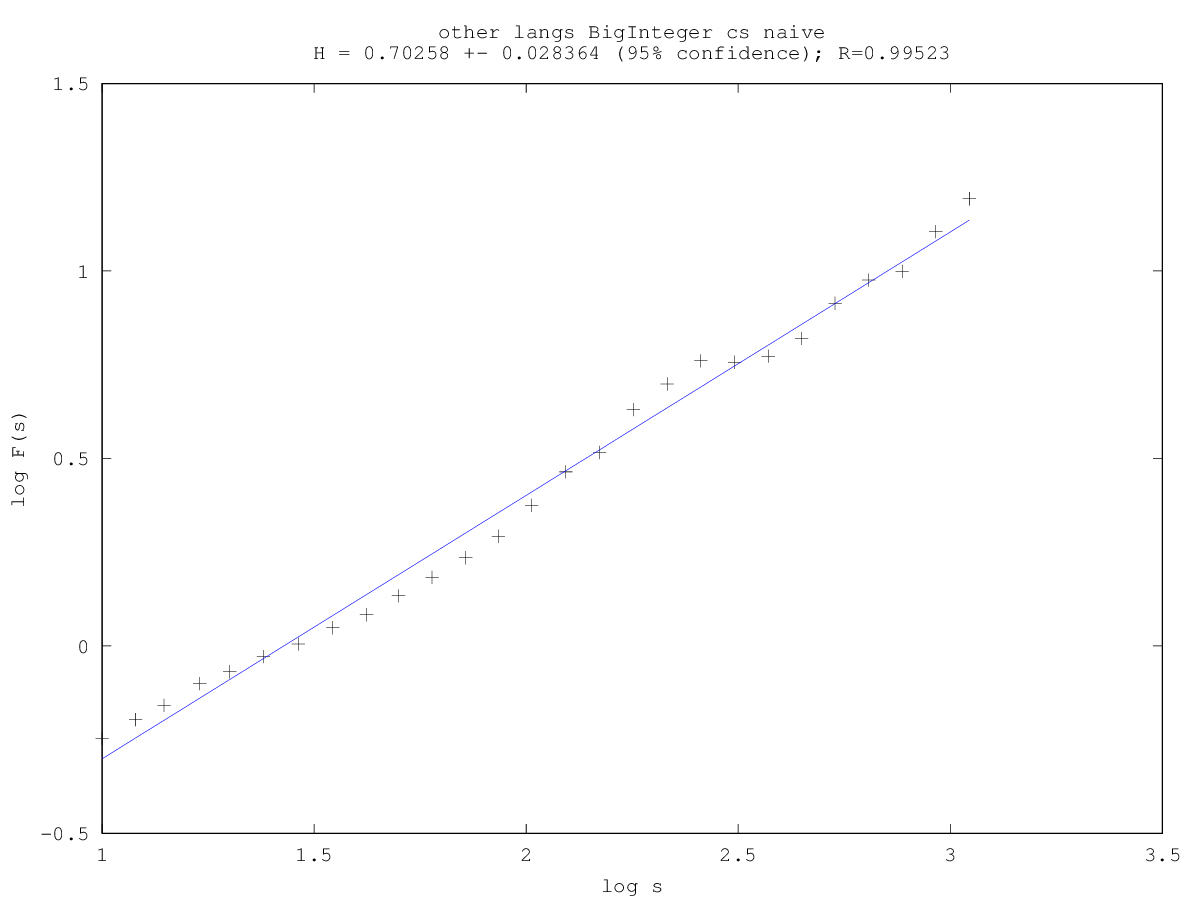
\includegraphics[width=0.8\linewidth]{{fractals/other_lang_data/other_langs_BigInteger_cs_naive_log_log}.png}
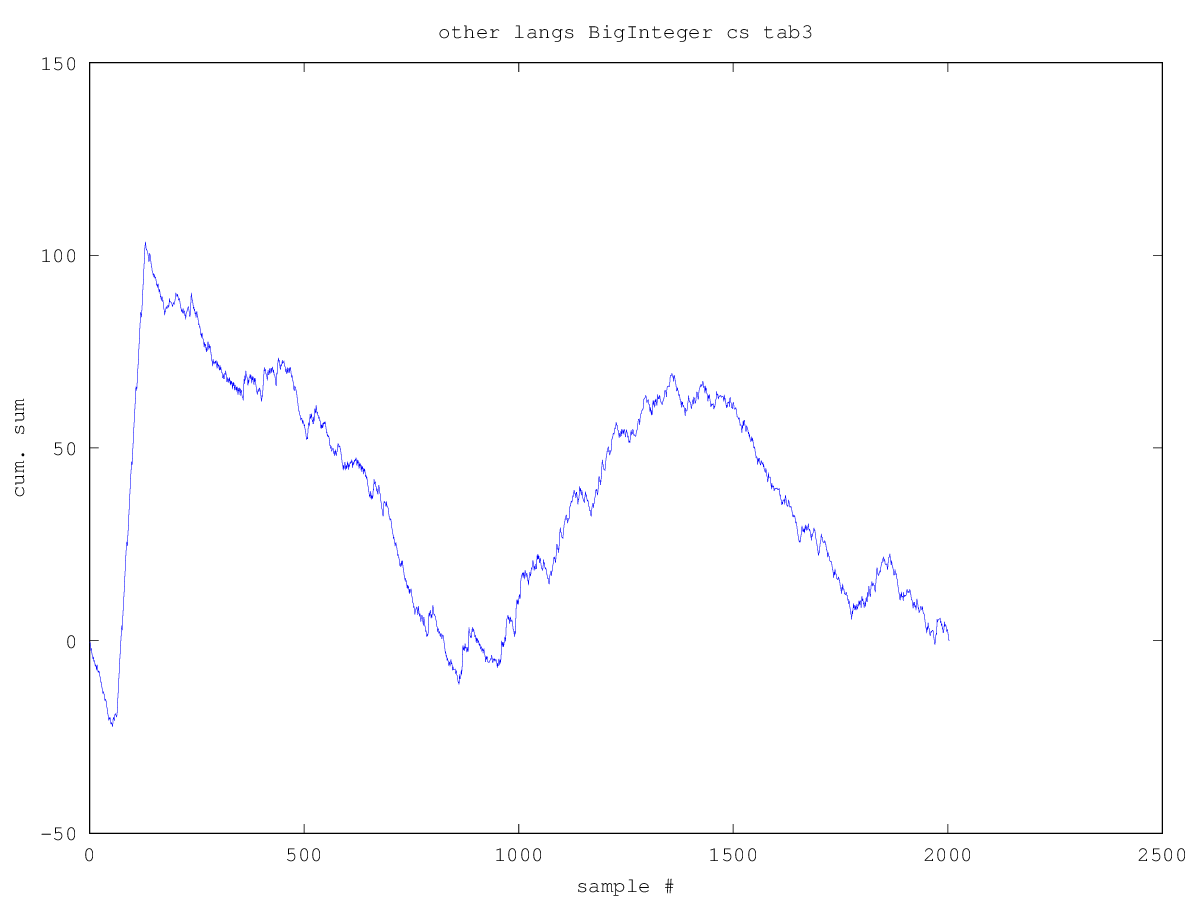
\includegraphics[width=0.8\linewidth]{{fractals/other_lang_data/other_langs_BigInteger_cs_tab3_time_series}.png}
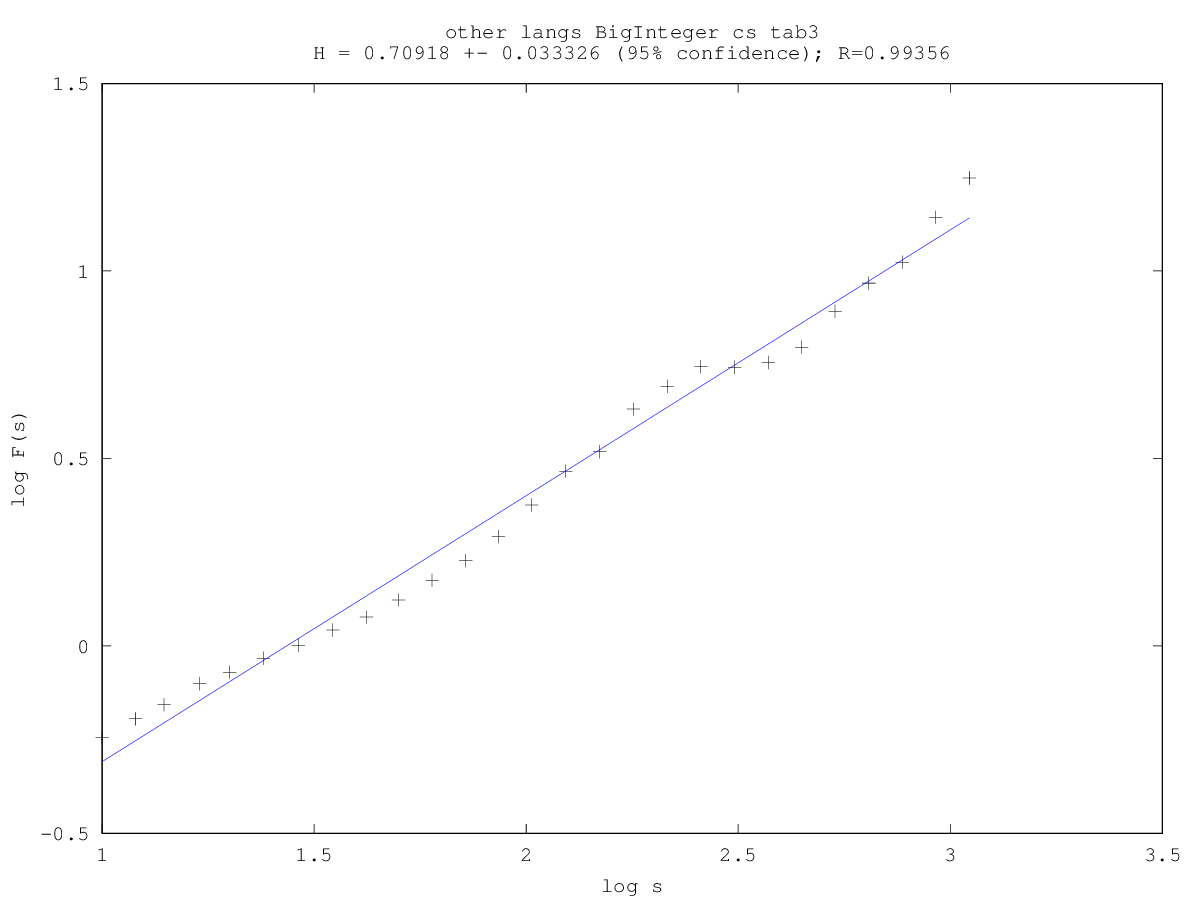
\includegraphics[width=0.8\linewidth]{{fractals/other_lang_data/other_langs_BigInteger_cs_tab3_log_log}.png}
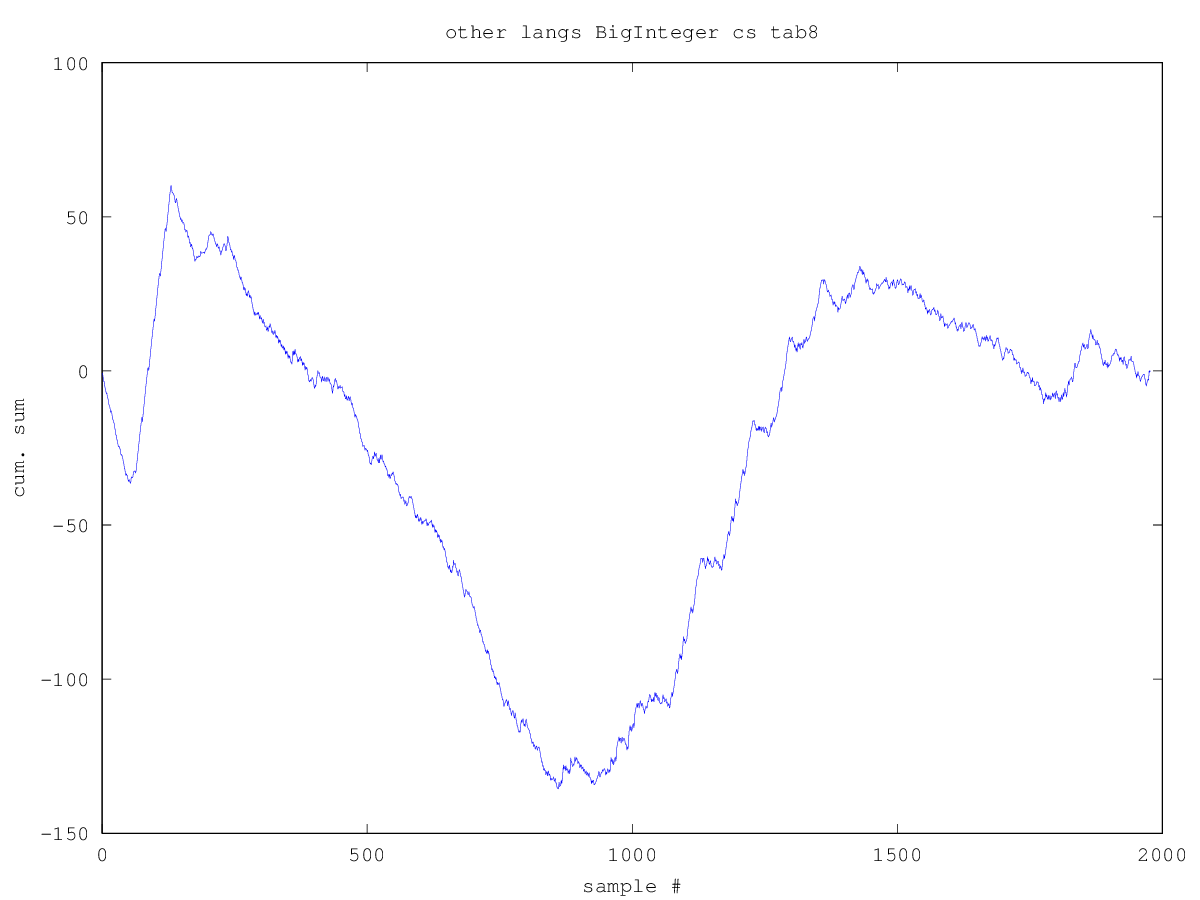
\includegraphics[width=0.8\linewidth]{{fractals/other_lang_data/other_langs_BigInteger_cs_tab8_time_series}.png}
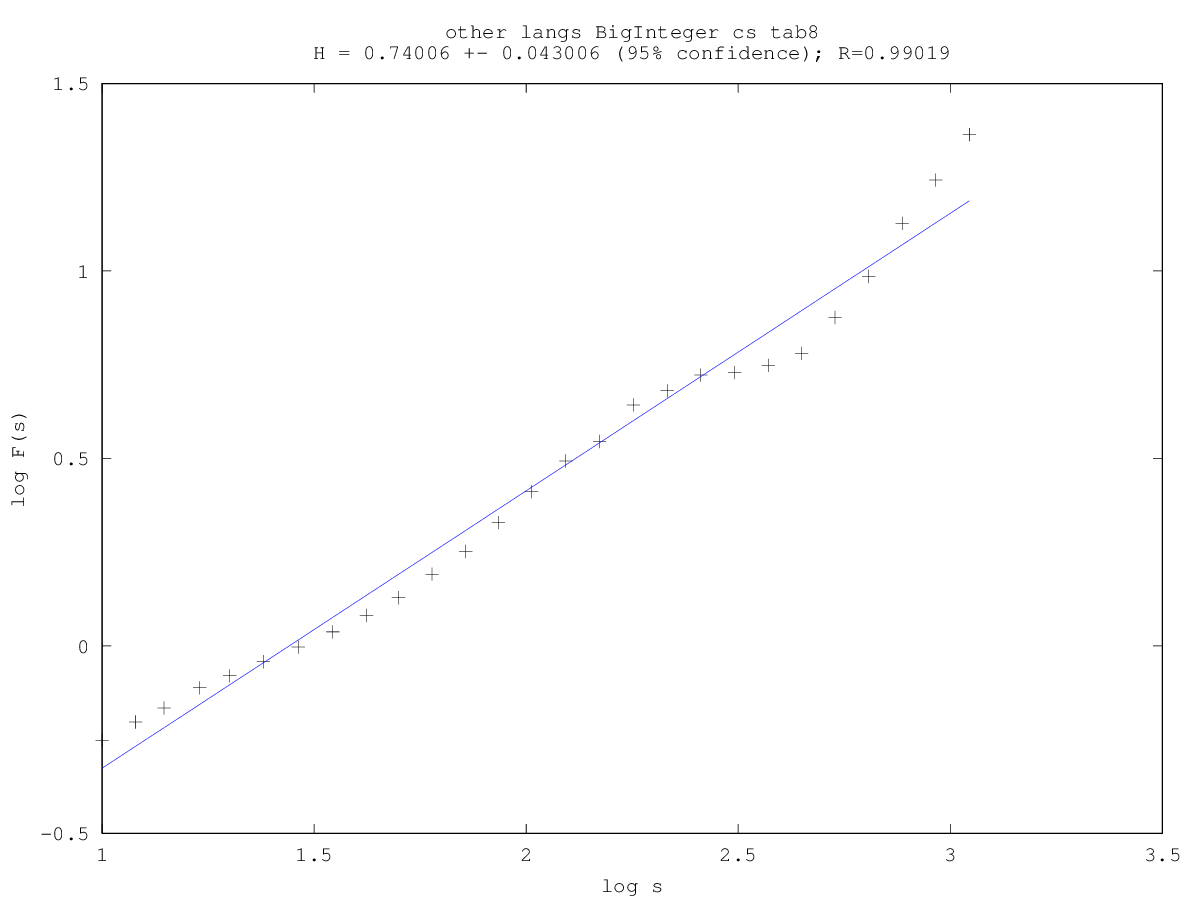
\includegraphics[width=0.8\linewidth]{{fractals/other_lang_data/other_langs_BigInteger_cs_tab8_log_log}.png}
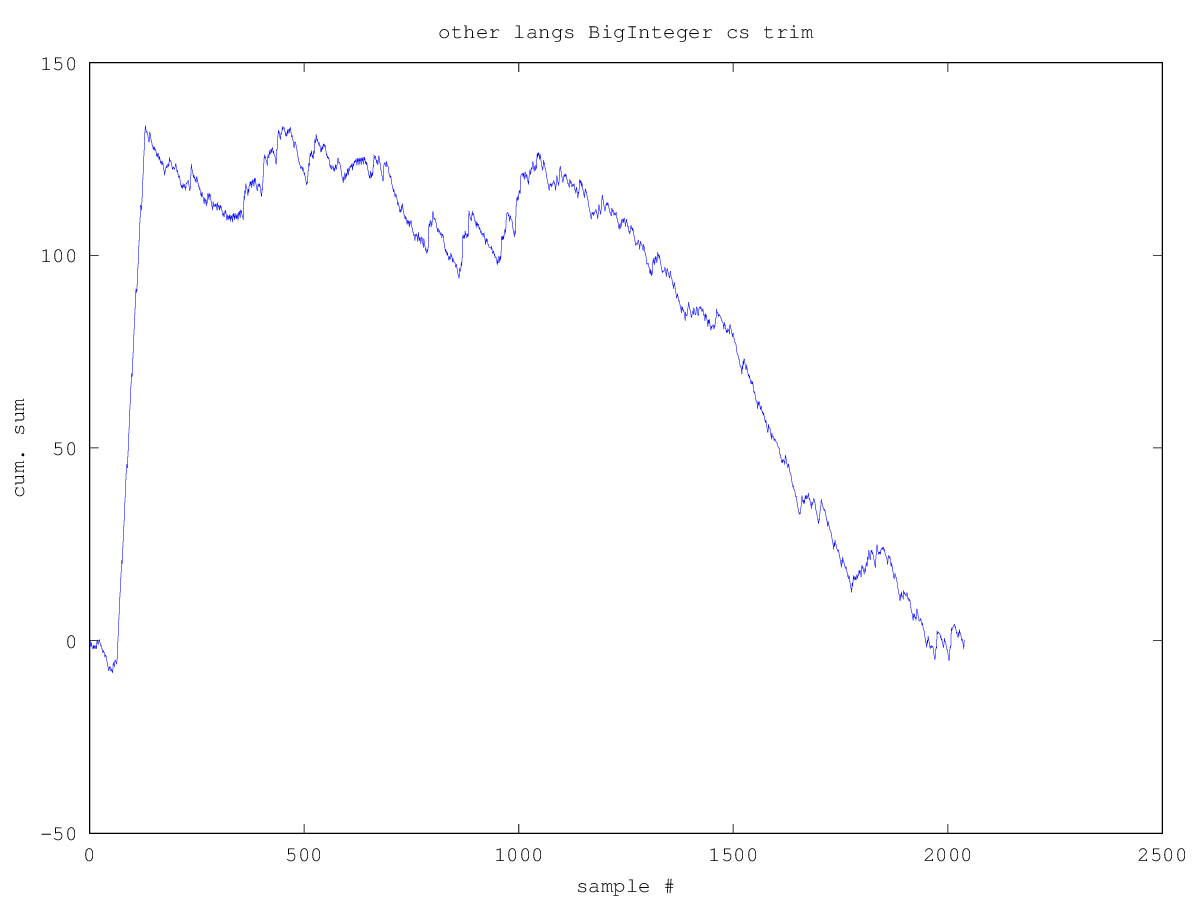
\includegraphics[width=0.8\linewidth]{{fractals/other_lang_data/other_langs_BigInteger_cs_trim_time_series}.png}
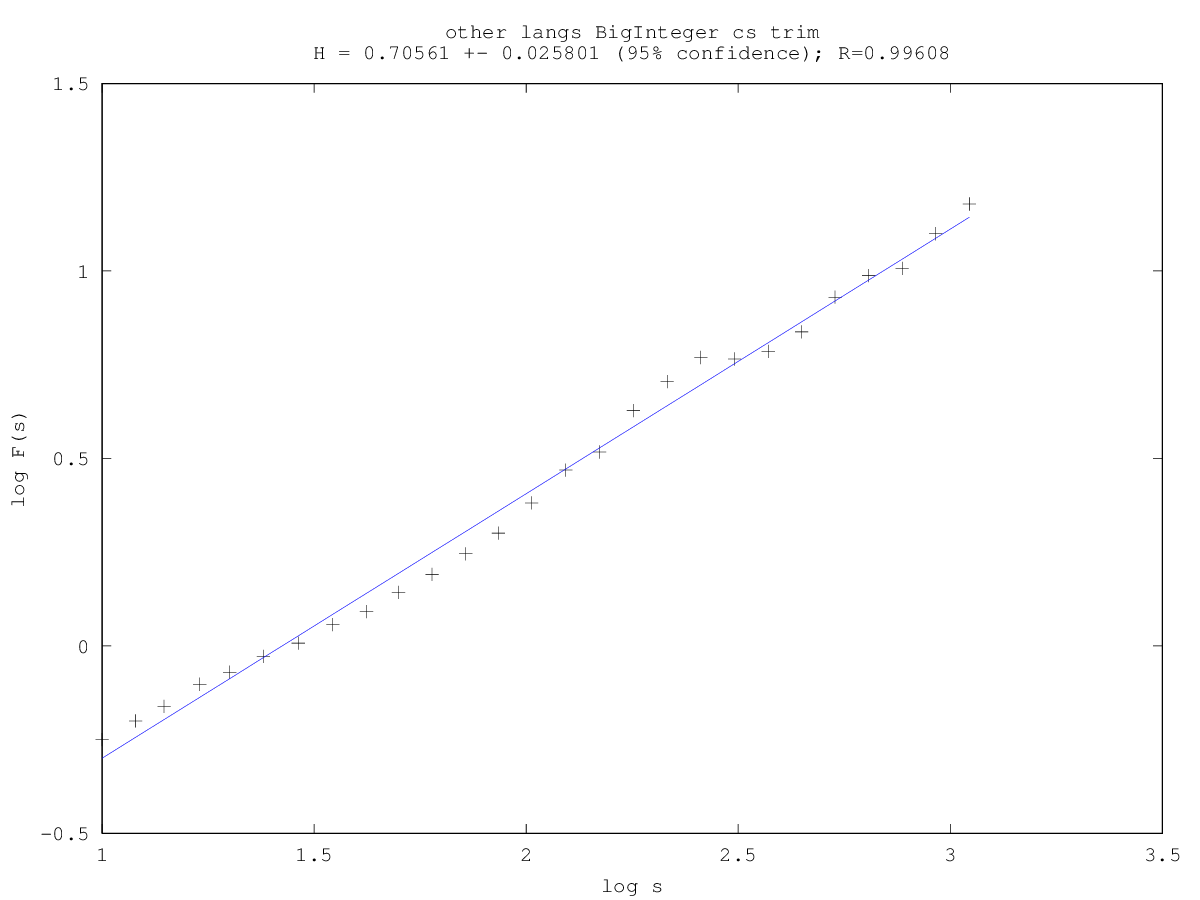
\includegraphics[width=0.8\linewidth]{{fractals/other_lang_data/other_langs_BigInteger_cs_trim_log_log}.png}
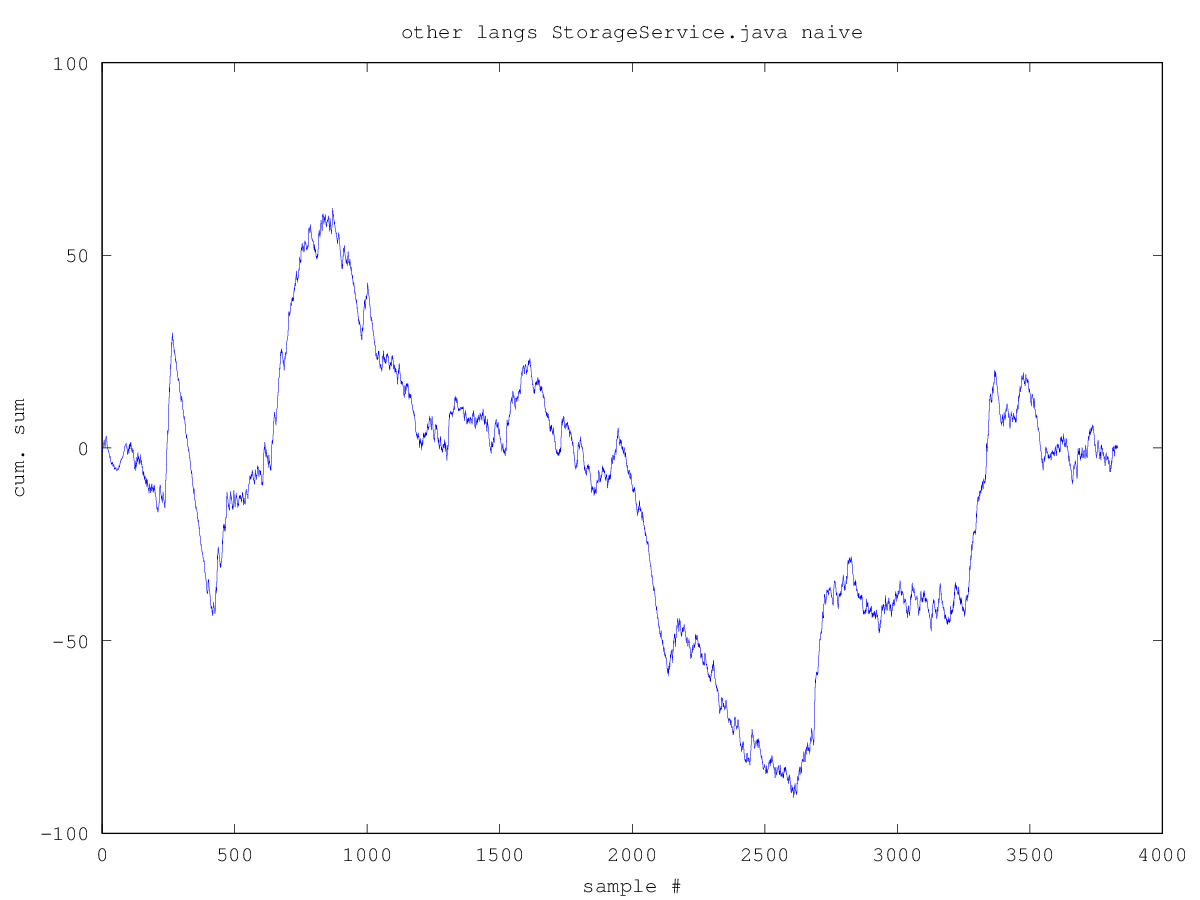
\includegraphics[width=0.8\linewidth]{{fractals/other_lang_data/other_langs_StorageService.java_naive_time_series}.png}
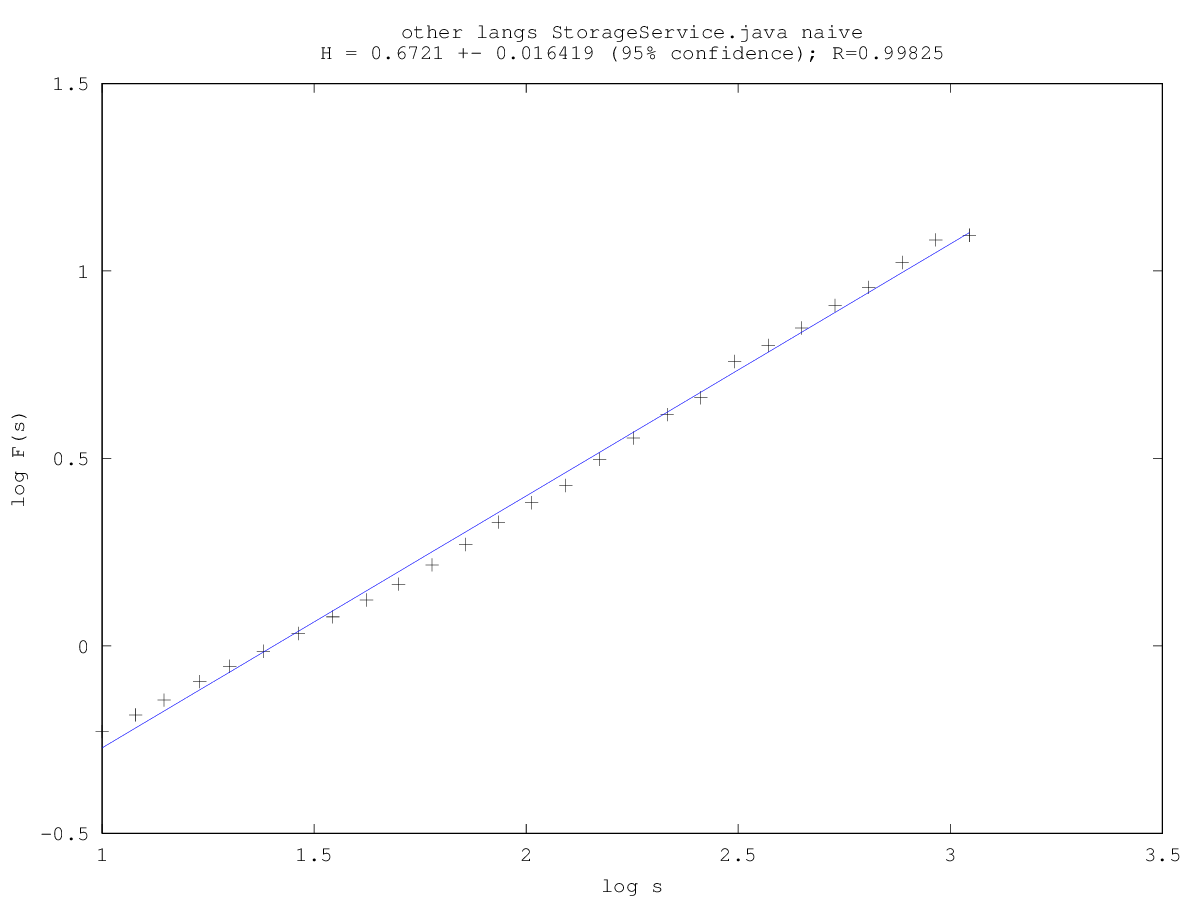
\includegraphics[width=0.8\linewidth]{{fractals/other_lang_data/other_langs_StorageService.java_naive_log_log}.png}
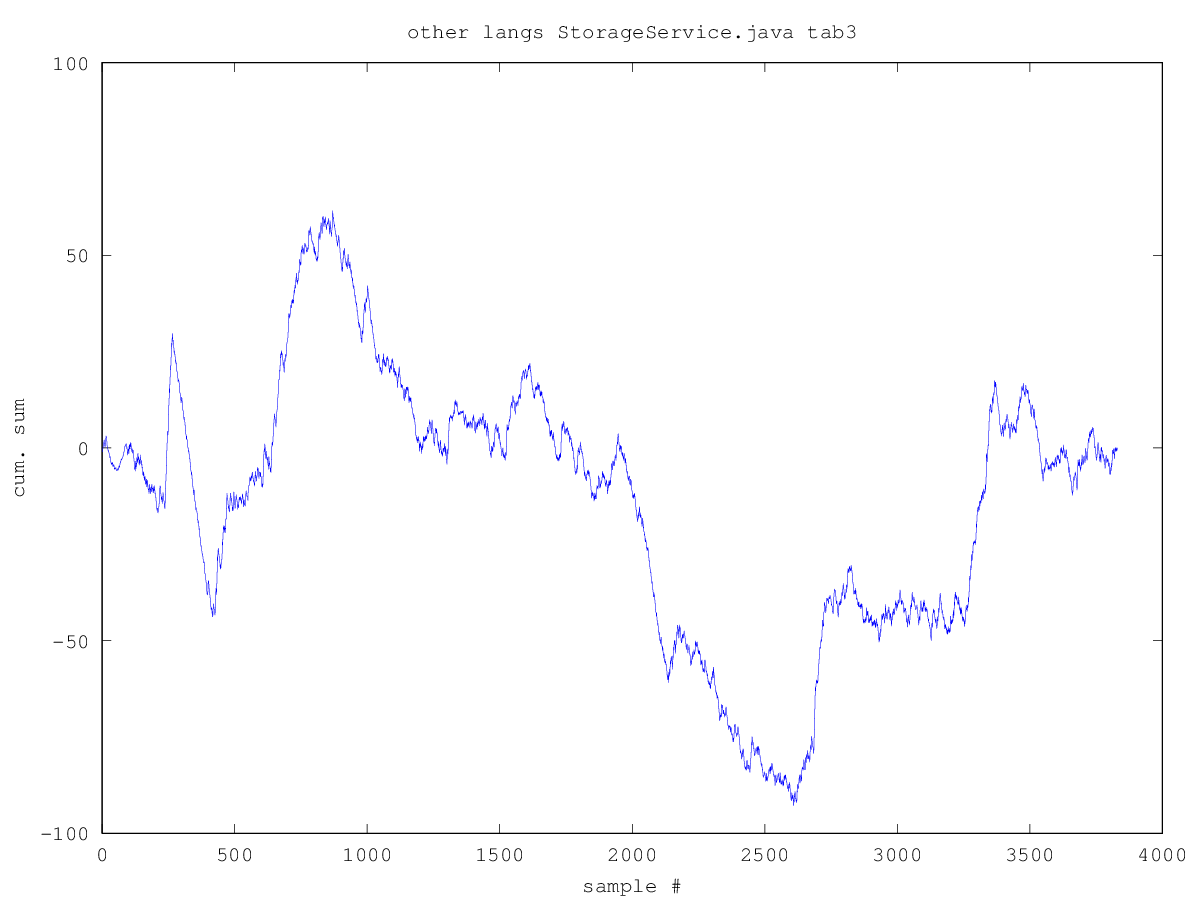
\includegraphics[width=0.8\linewidth]{{fractals/other_lang_data/other_langs_StorageService.java_tab3_time_series}.png}
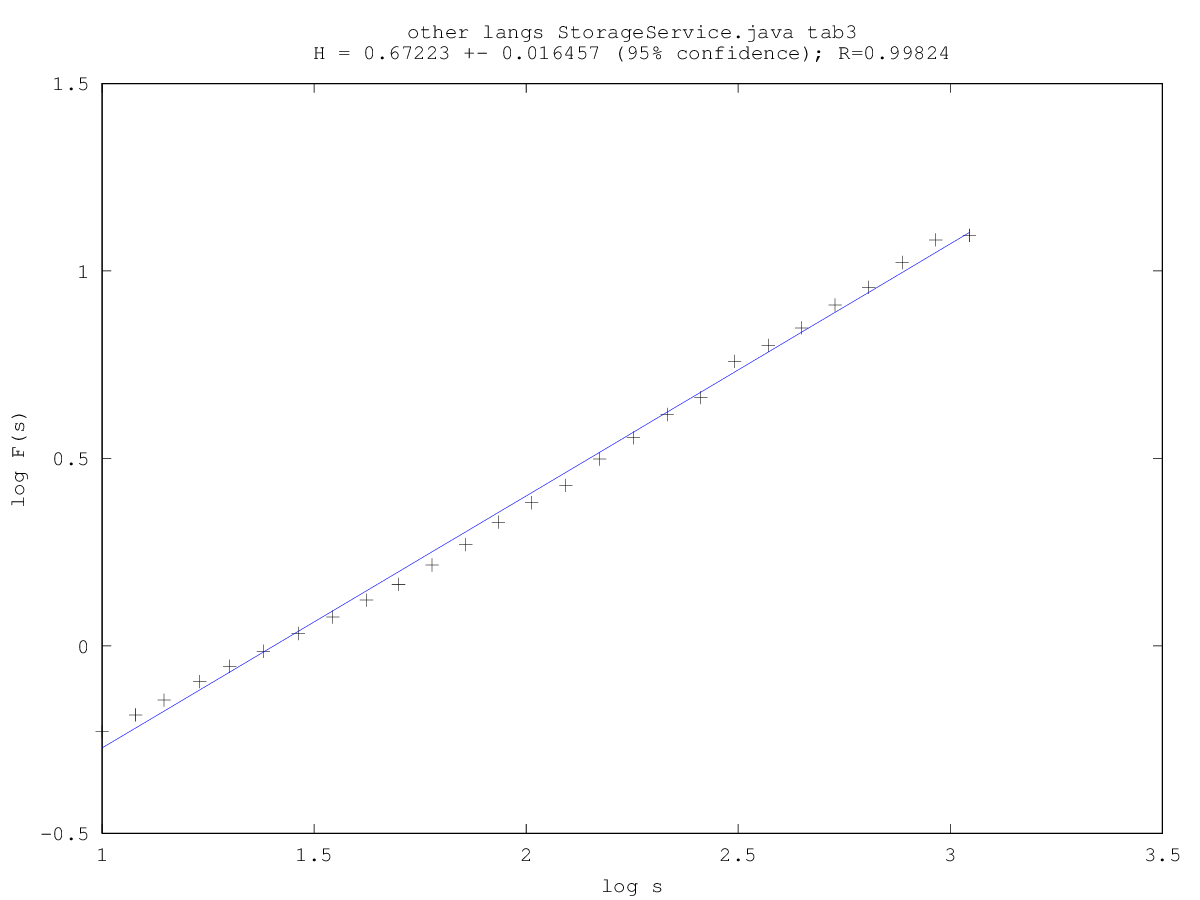
\includegraphics[width=0.8\linewidth]{{fractals/other_lang_data/other_langs_StorageService.java_tab3_log_log}.png}
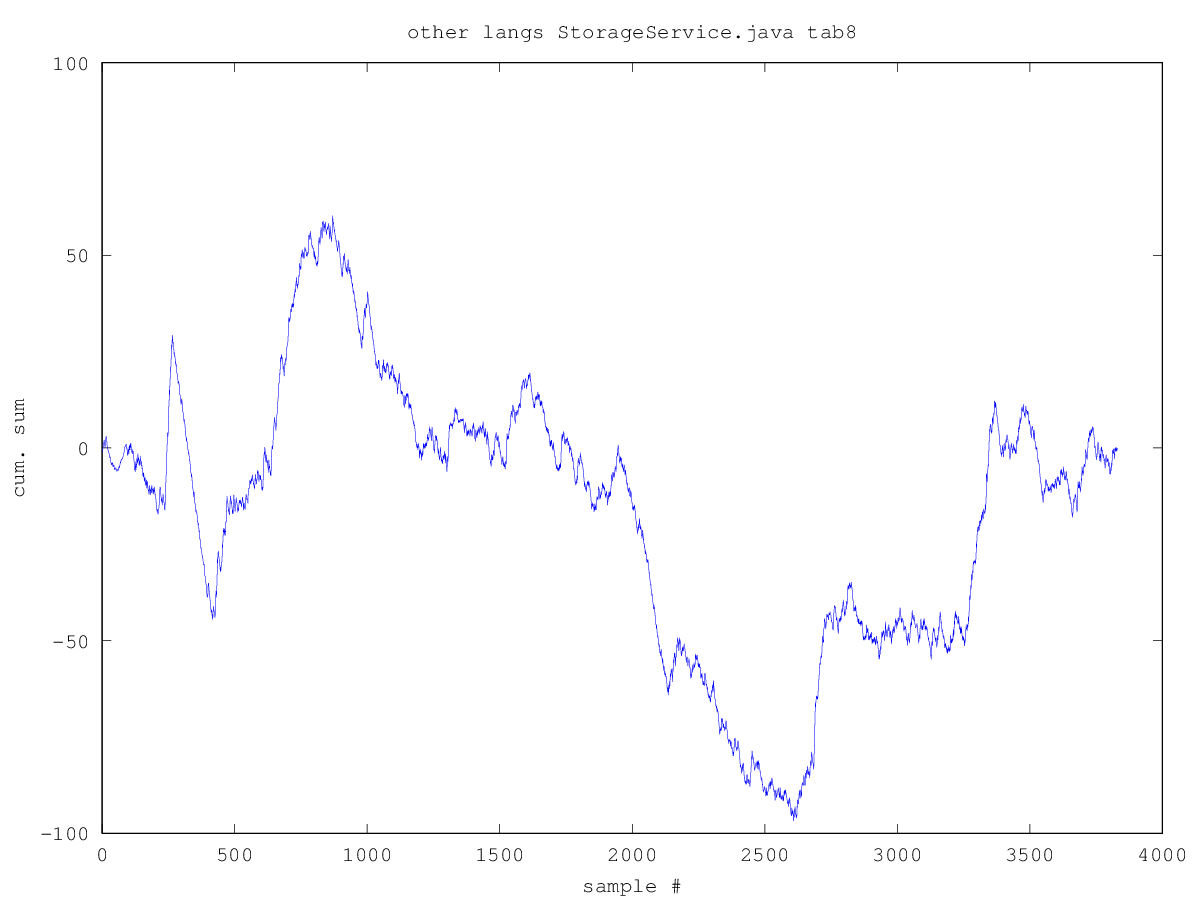
\includegraphics[width=0.8\linewidth]{{fractals/other_lang_data/other_langs_StorageService.java_tab8_time_series}.png}
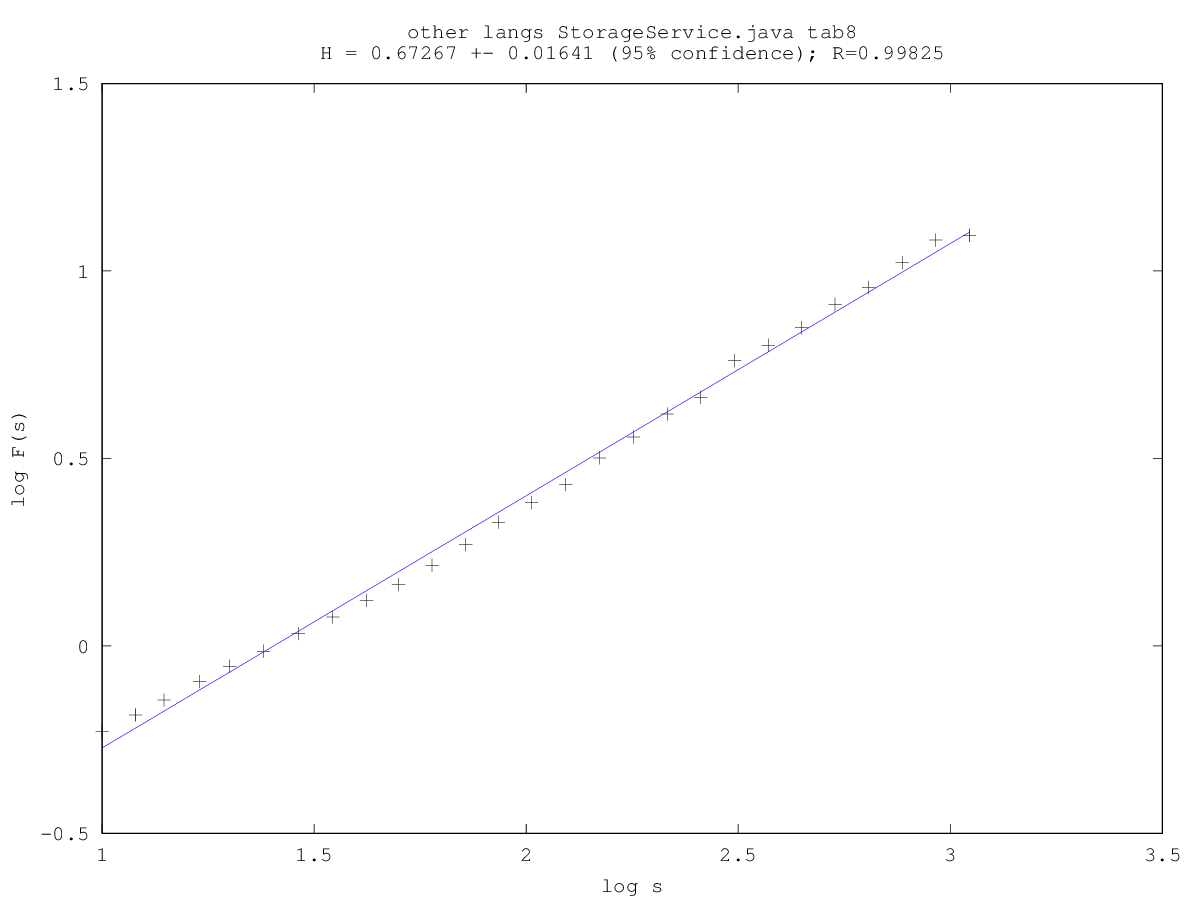
\includegraphics[width=0.8\linewidth]{{fractals/other_lang_data/other_langs_StorageService.java_tab8_log_log}.png}
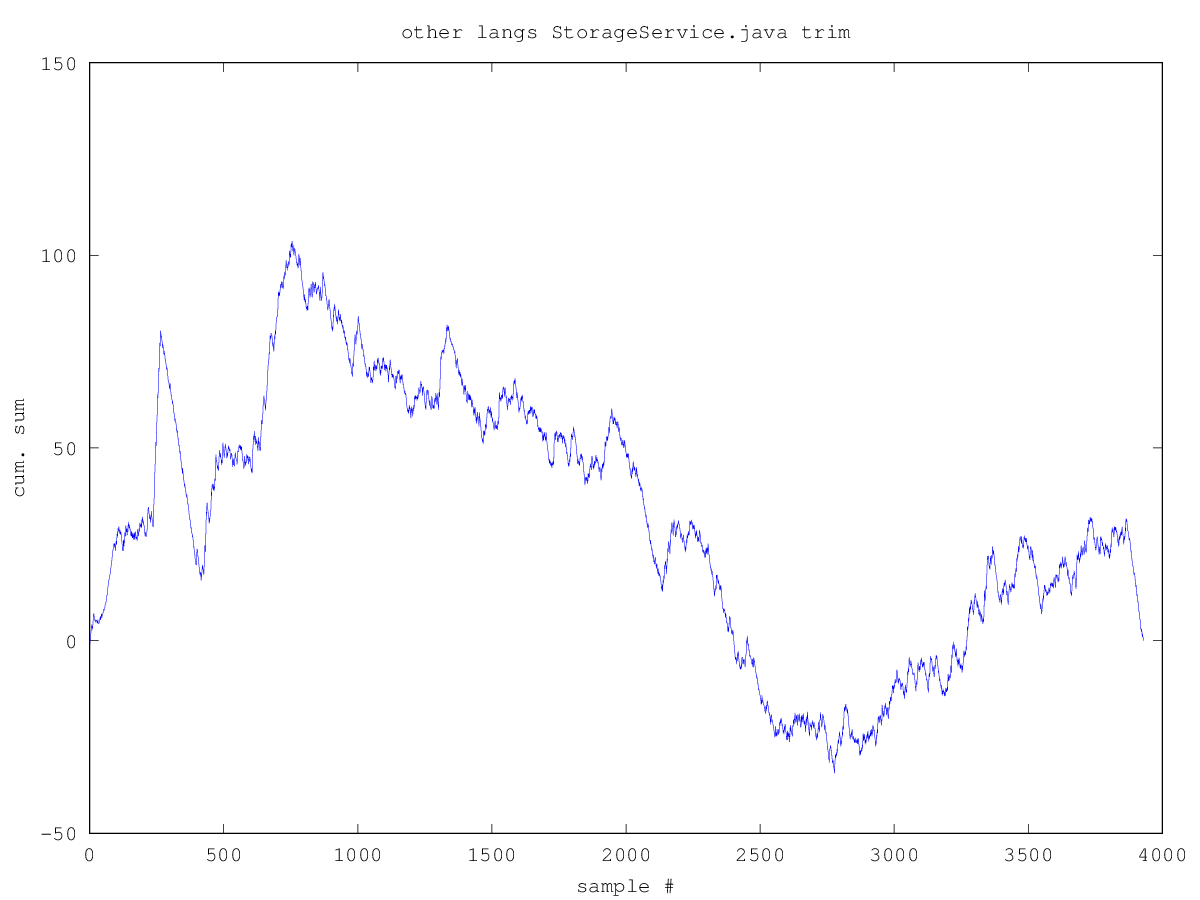
\includegraphics[width=0.8\linewidth]{{fractals/other_lang_data/other_langs_StorageService.java_trim_time_series}.png}
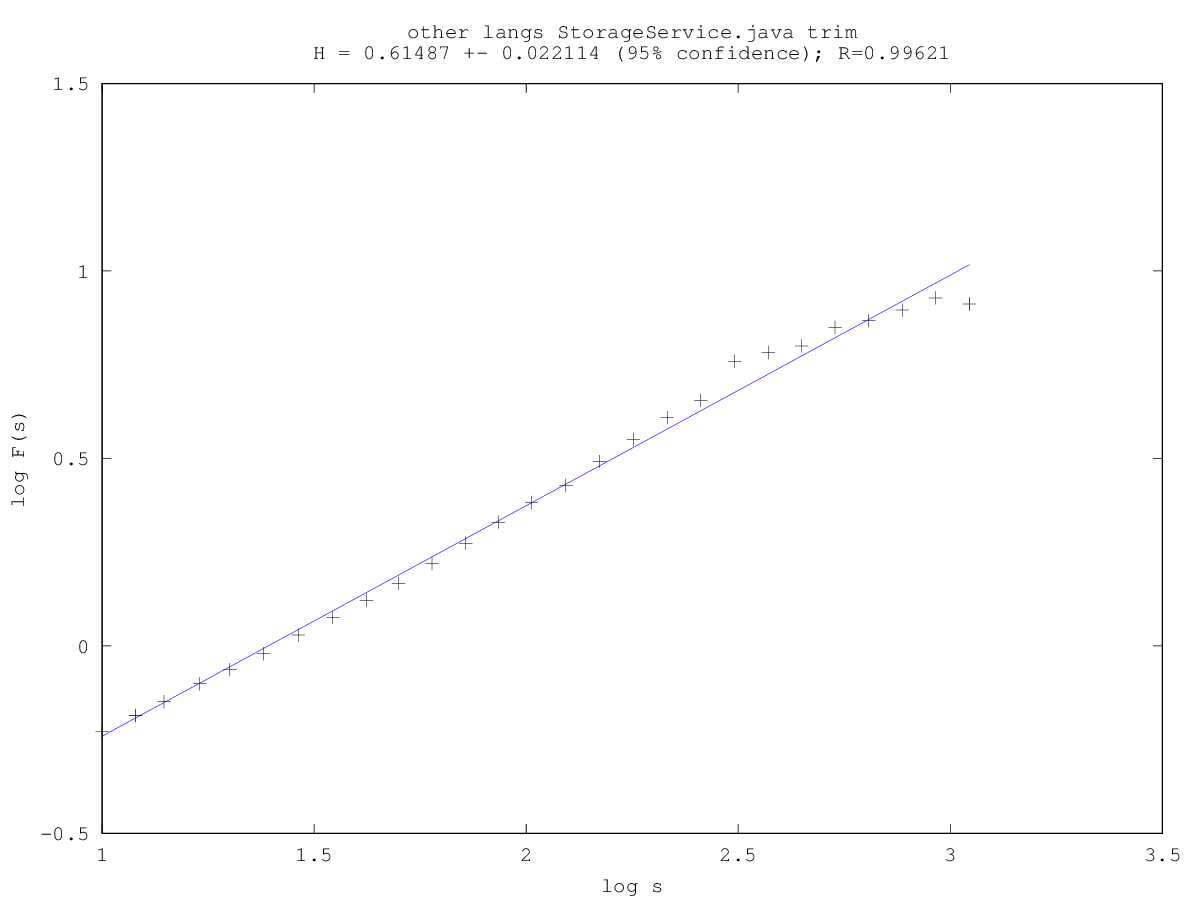
\includegraphics[width=0.8\linewidth]{{fractals/other_lang_data/other_langs_StorageService.java_trim_log_log}.png}
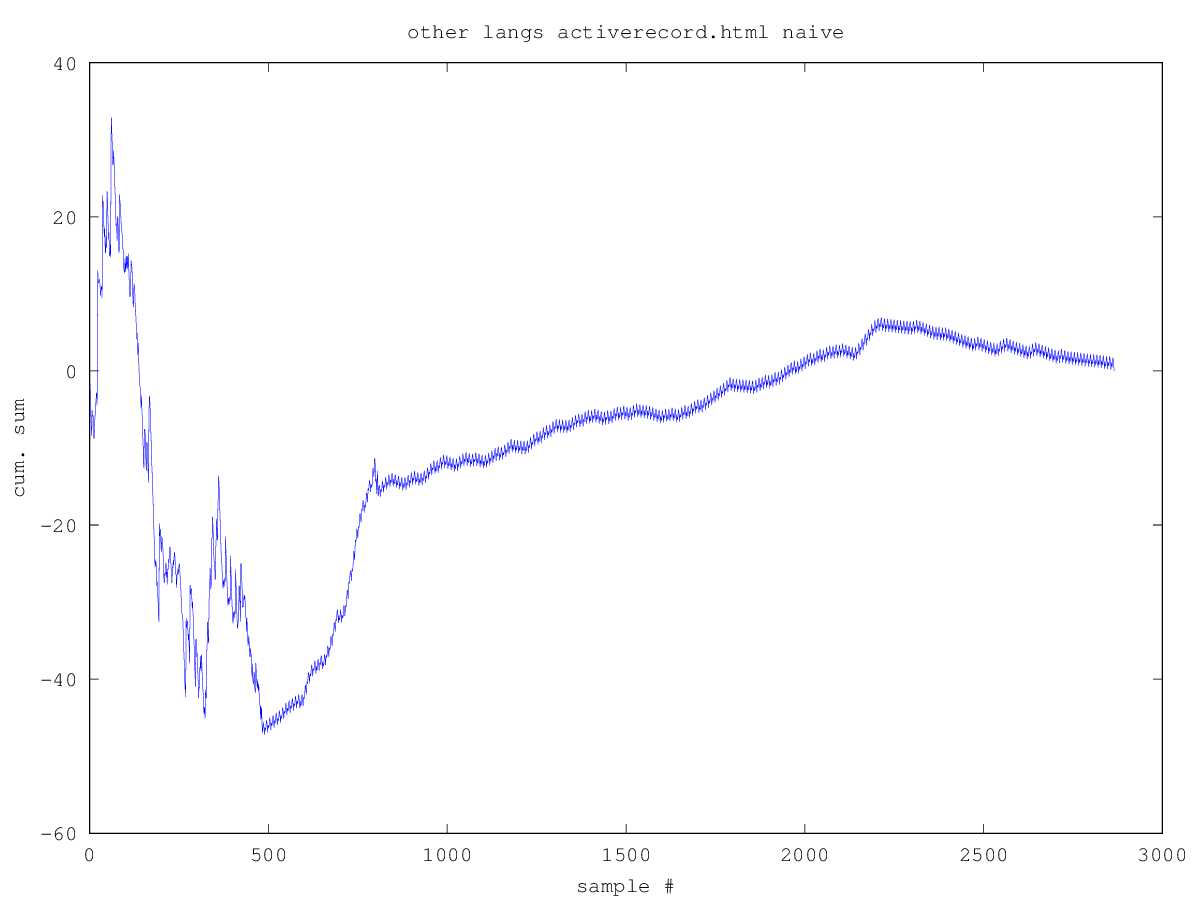
\includegraphics[width=0.8\linewidth]{{fractals/other_lang_data/other_langs_activerecord.html_naive_time_series}.png}
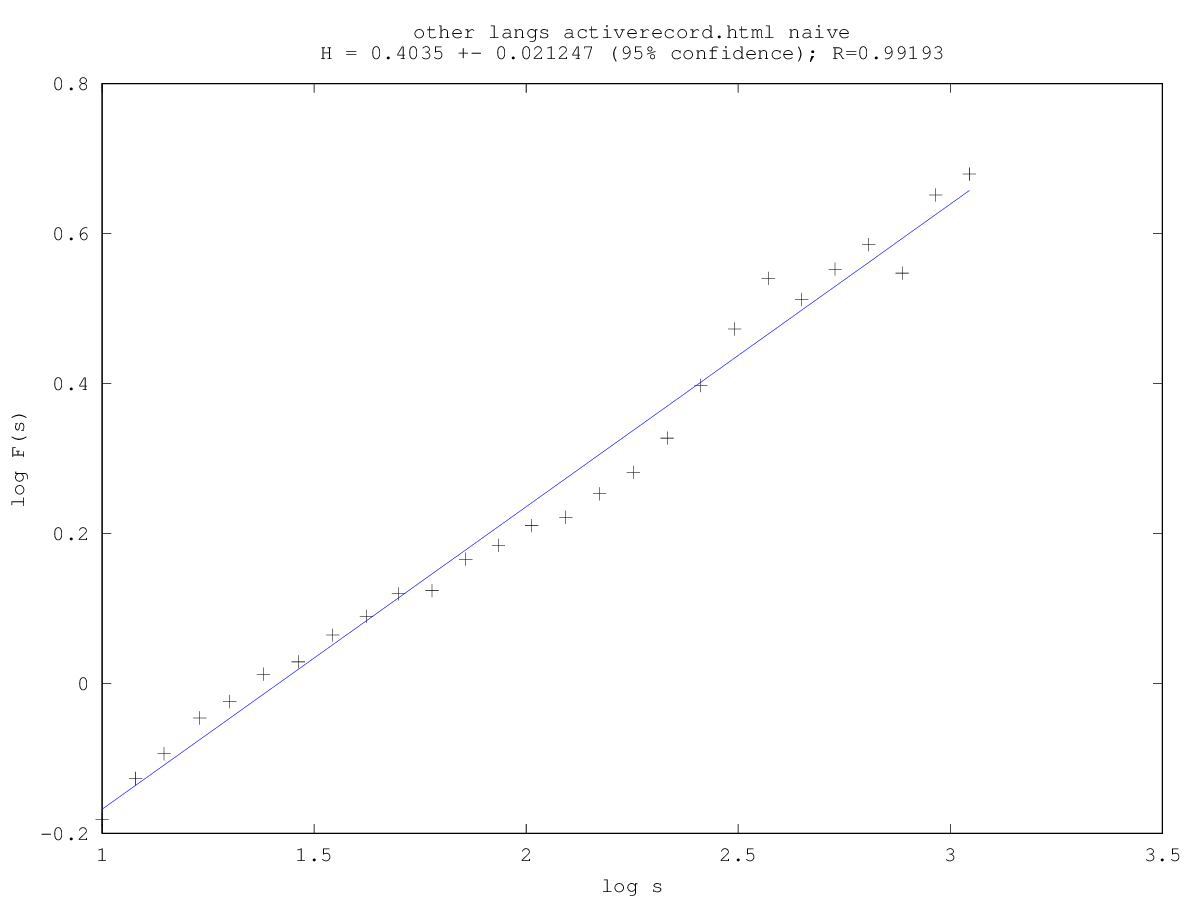
\includegraphics[width=0.8\linewidth]{{fractals/other_lang_data/other_langs_activerecord.html_naive_log_log}.png}
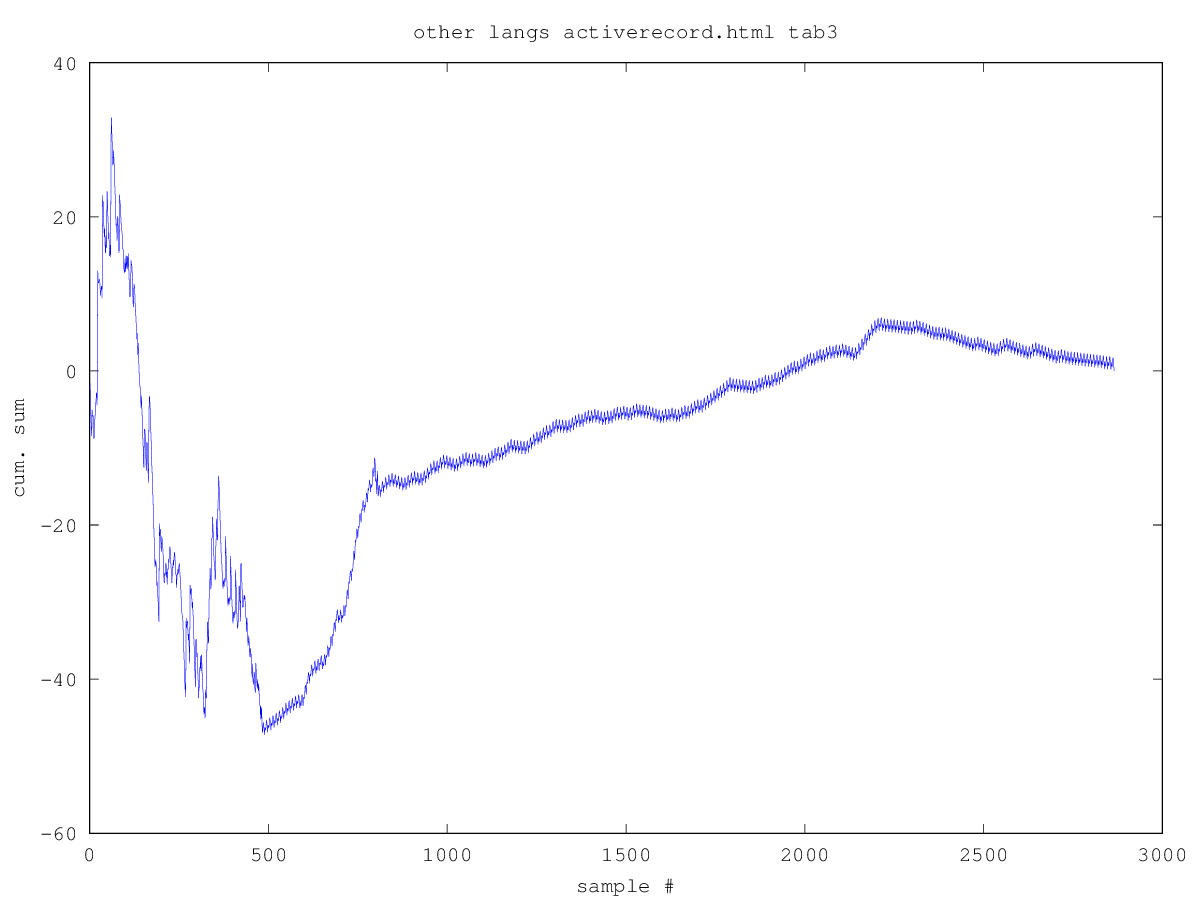
\includegraphics[width=0.8\linewidth]{{fractals/other_lang_data/other_langs_activerecord.html_tab3_time_series}.png}
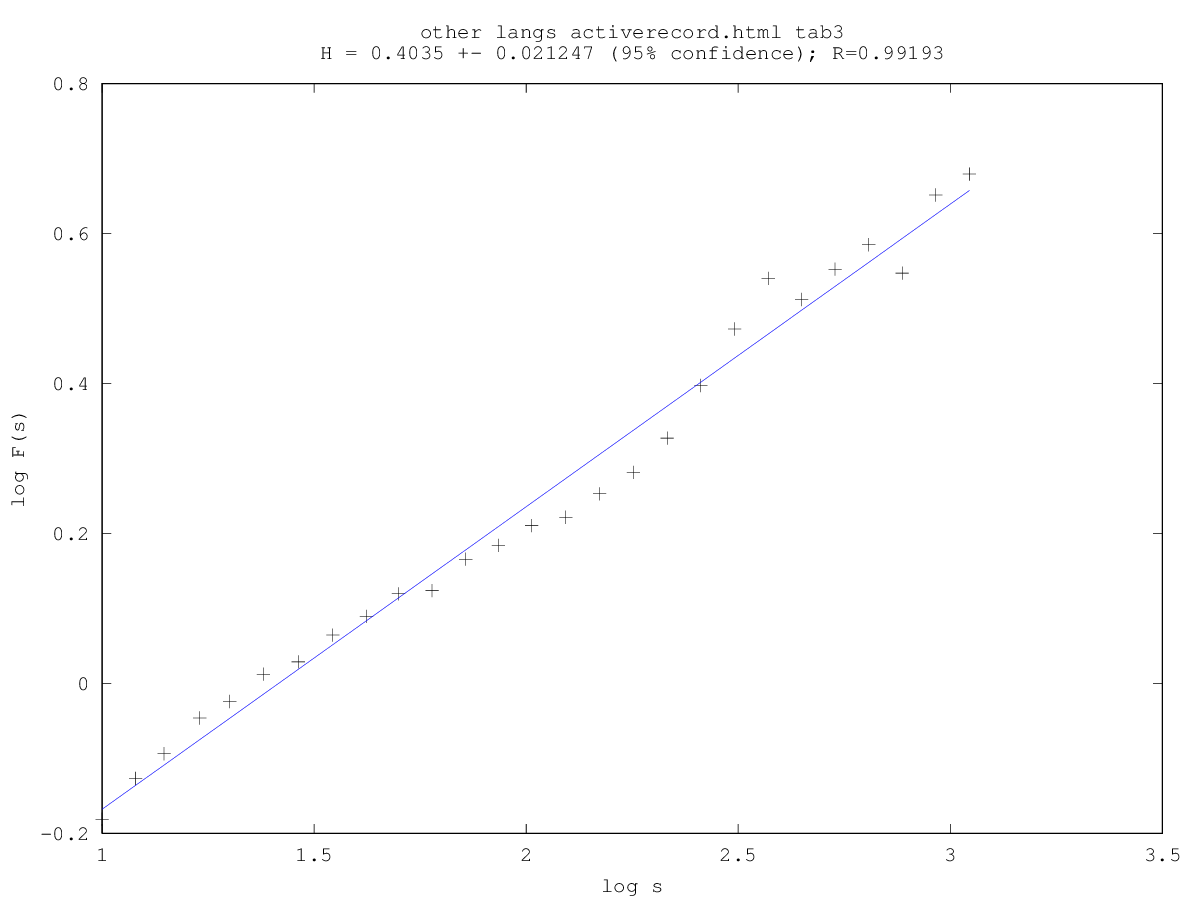
\includegraphics[width=0.8\linewidth]{{fractals/other_lang_data/other_langs_activerecord.html_tab3_log_log}.png}
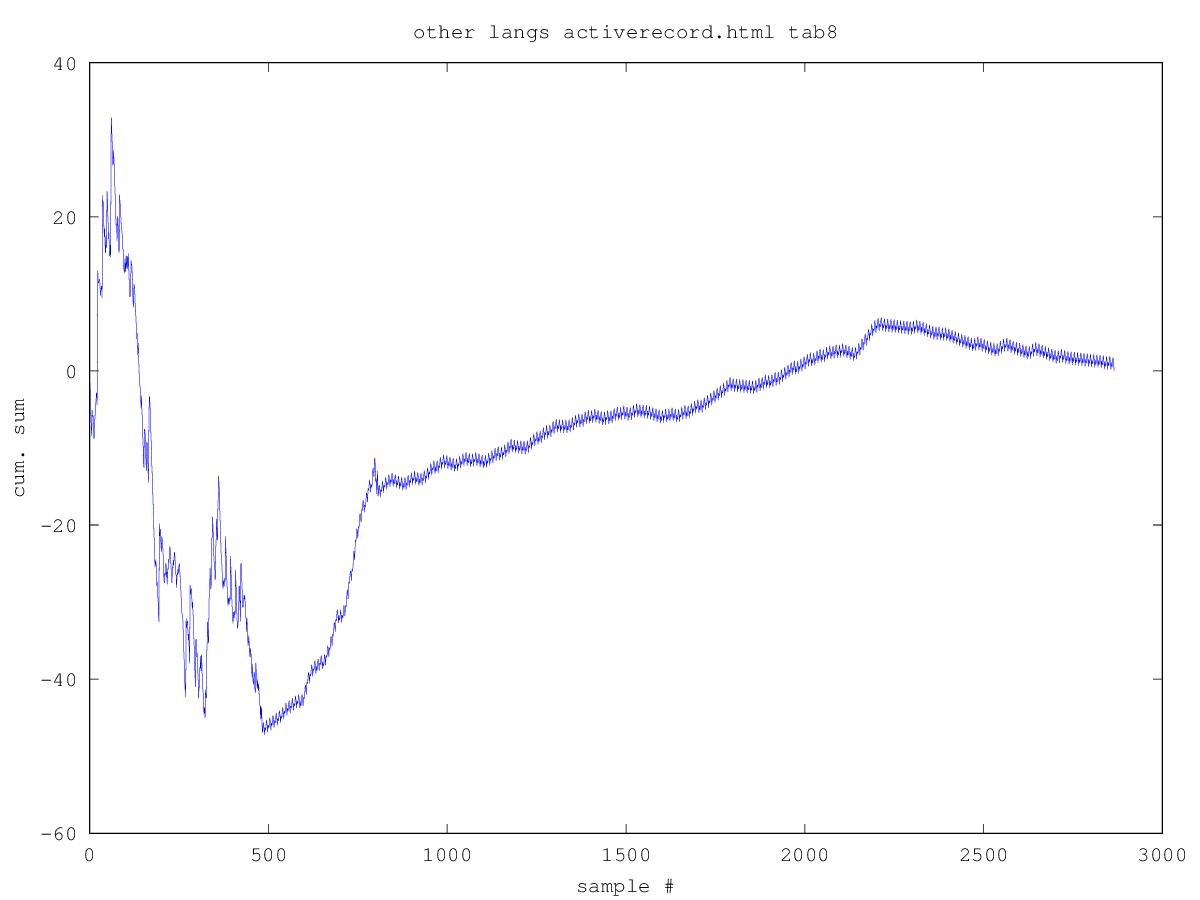
\includegraphics[width=0.8\linewidth]{{fractals/other_lang_data/other_langs_activerecord.html_tab8_time_series}.png}
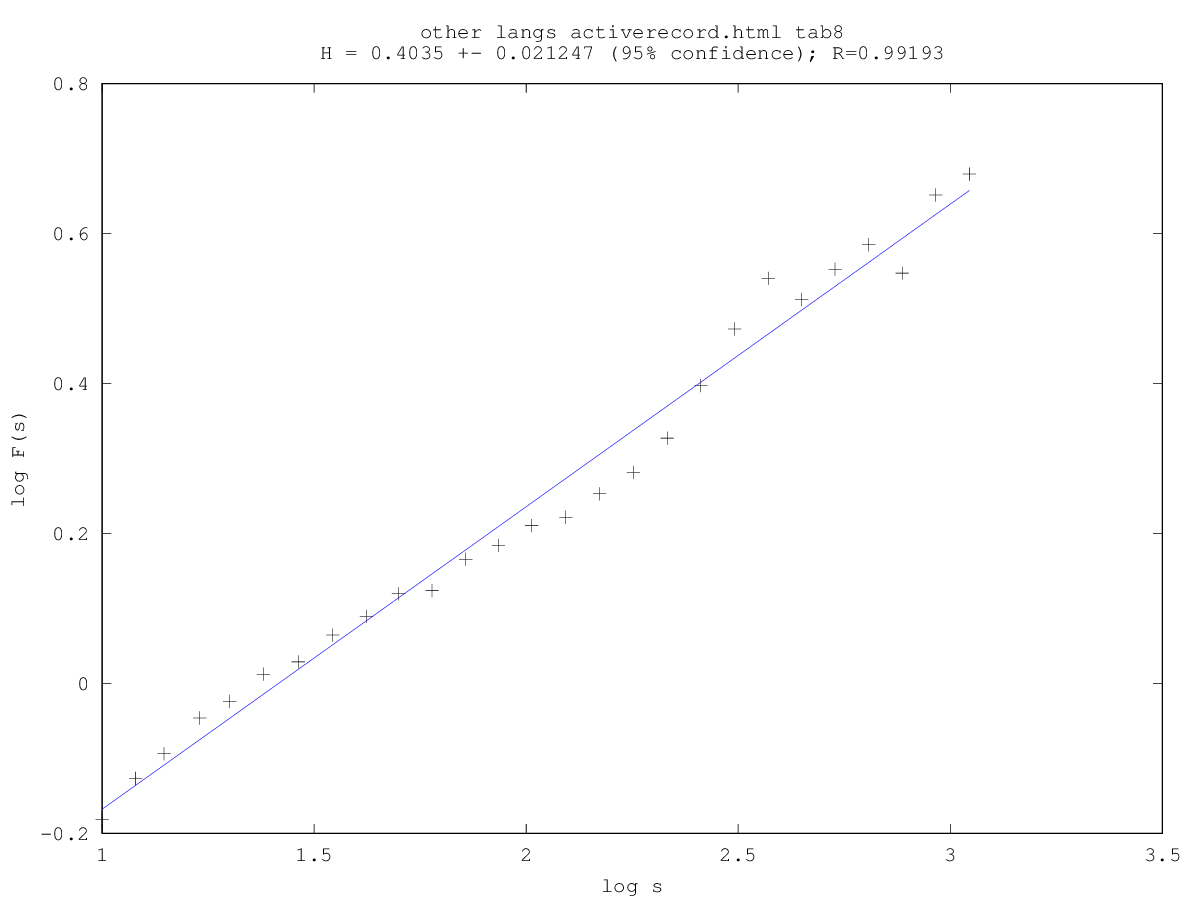
\includegraphics[width=0.8\linewidth]{{fractals/other_lang_data/other_langs_activerecord.html_tab8_log_log}.png}
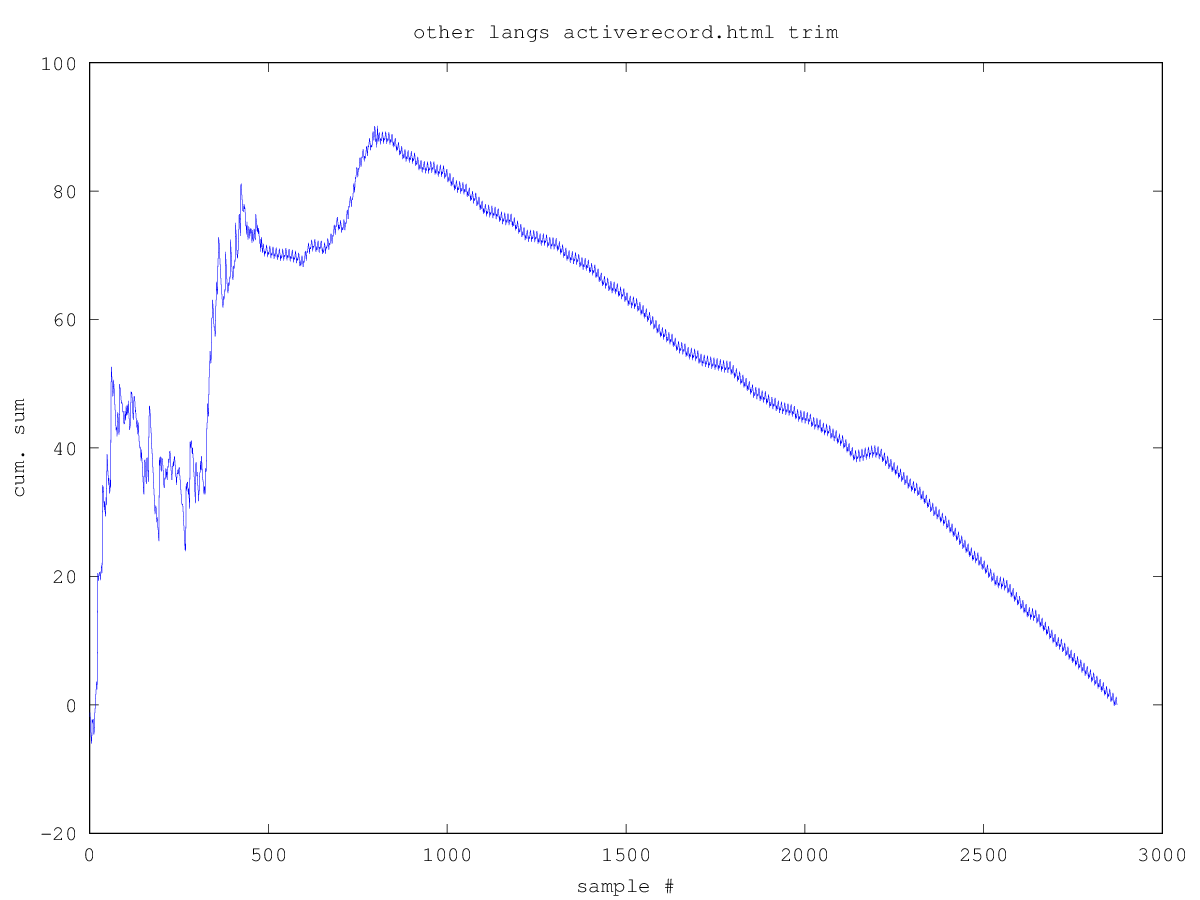
\includegraphics[width=0.8\linewidth]{{fractals/other_lang_data/other_langs_activerecord.html_trim_time_series}.png}
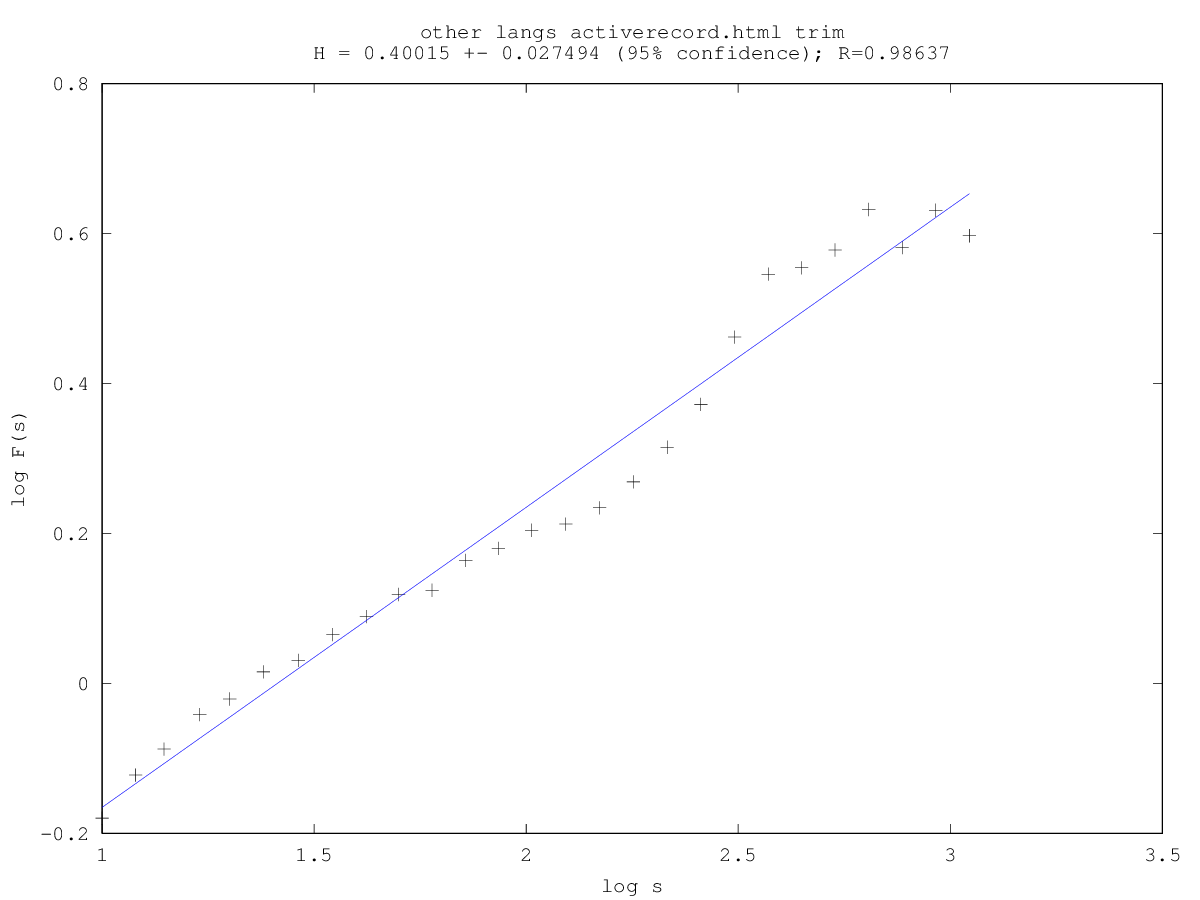
\includegraphics[width=0.8\linewidth]{{fractals/other_lang_data/other_langs_activerecord.html_trim_log_log}.png}
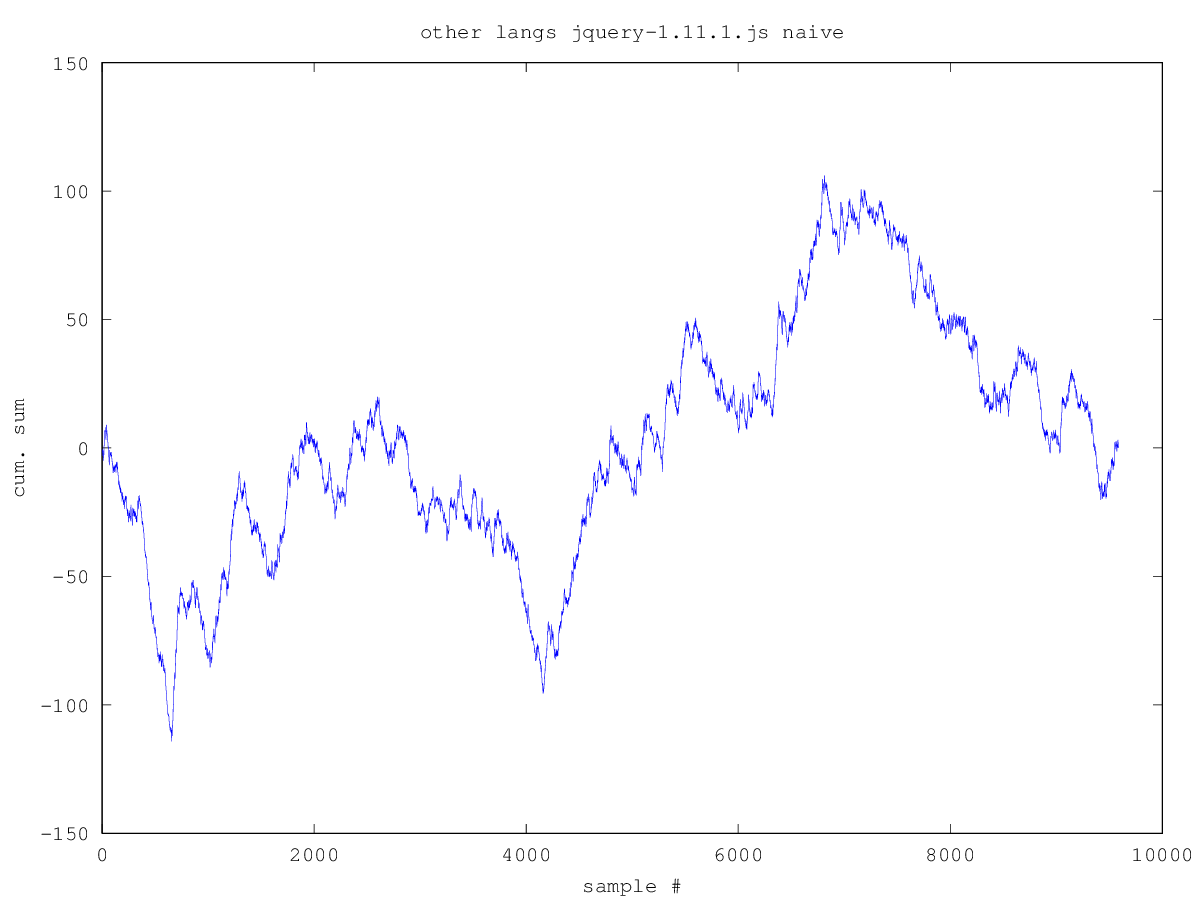
\includegraphics[width=0.8\linewidth]{{fractals/other_lang_data/other_langs_jquery-1.11.1.js_naive_time_series}.png}
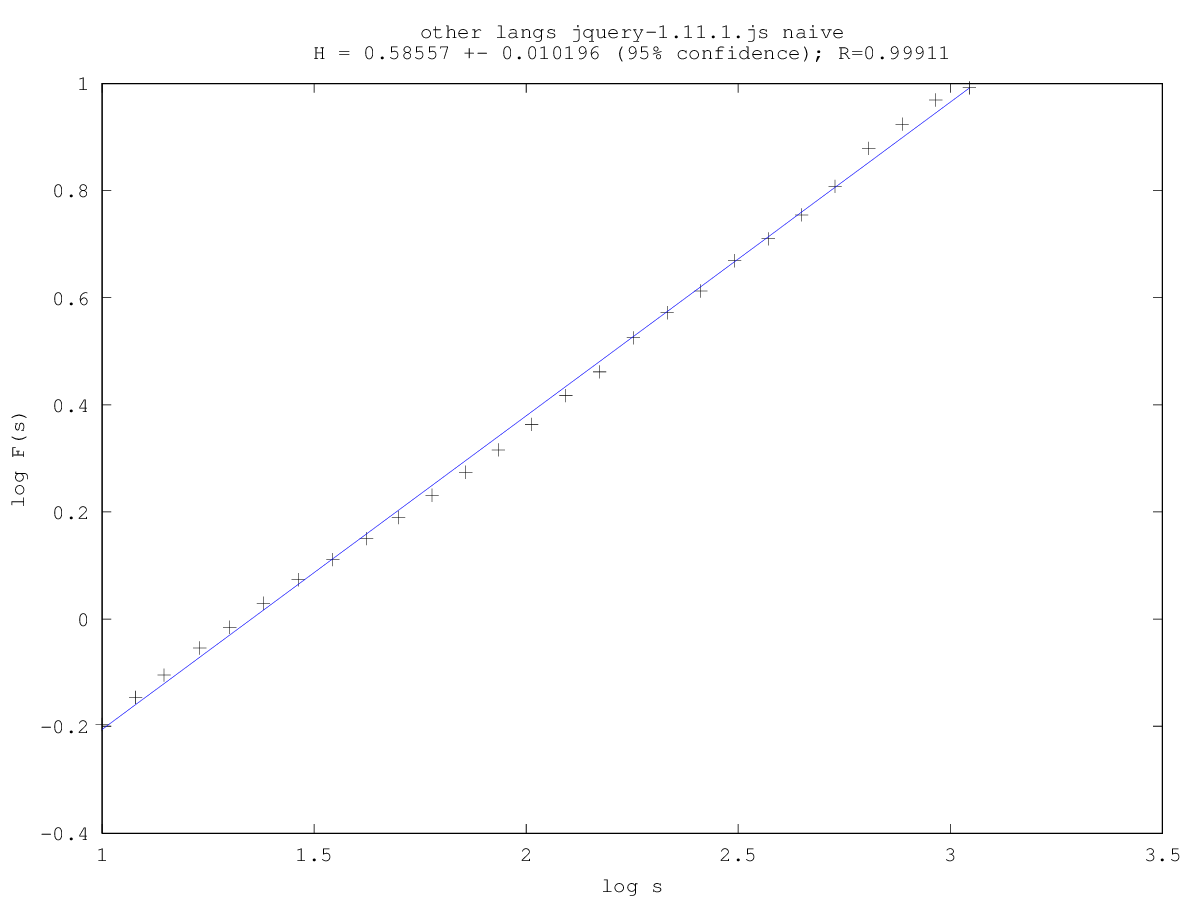
\includegraphics[width=0.8\linewidth]{{fractals/other_lang_data/other_langs_jquery-1.11.1.js_naive_log_log}.png}
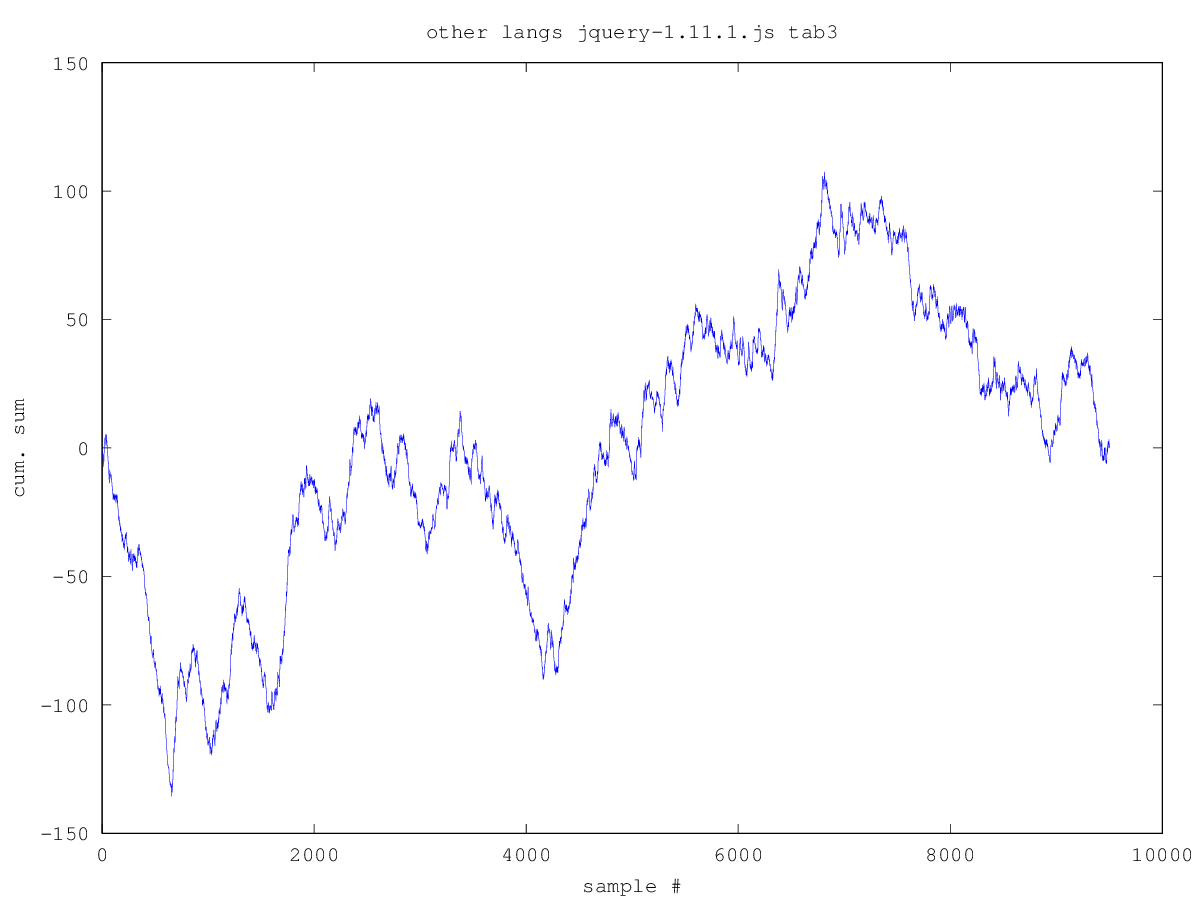
\includegraphics[width=0.8\linewidth]{{fractals/other_lang_data/other_langs_jquery-1.11.1.js_tab3_time_series}.png}
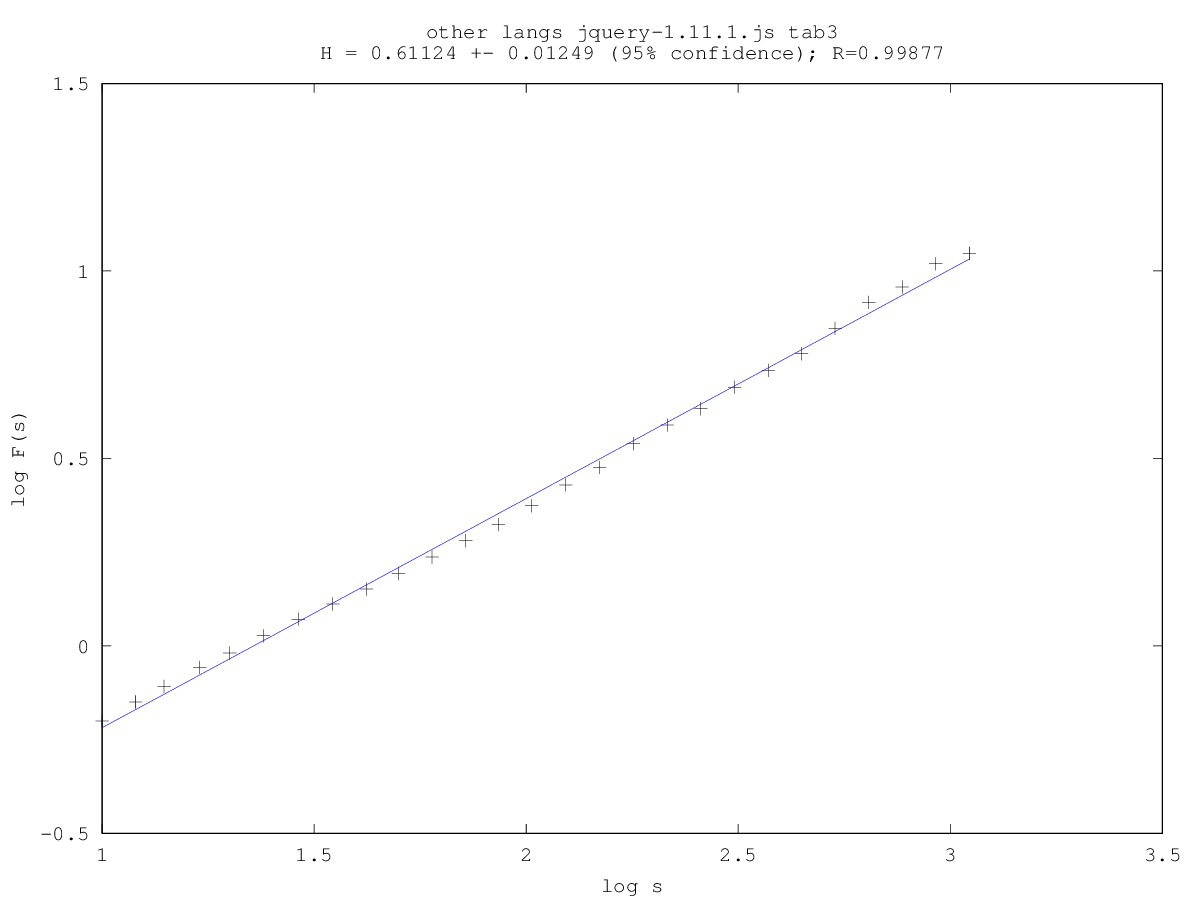
\includegraphics[width=0.8\linewidth]{{fractals/other_lang_data/other_langs_jquery-1.11.1.js_tab3_log_log}.png}
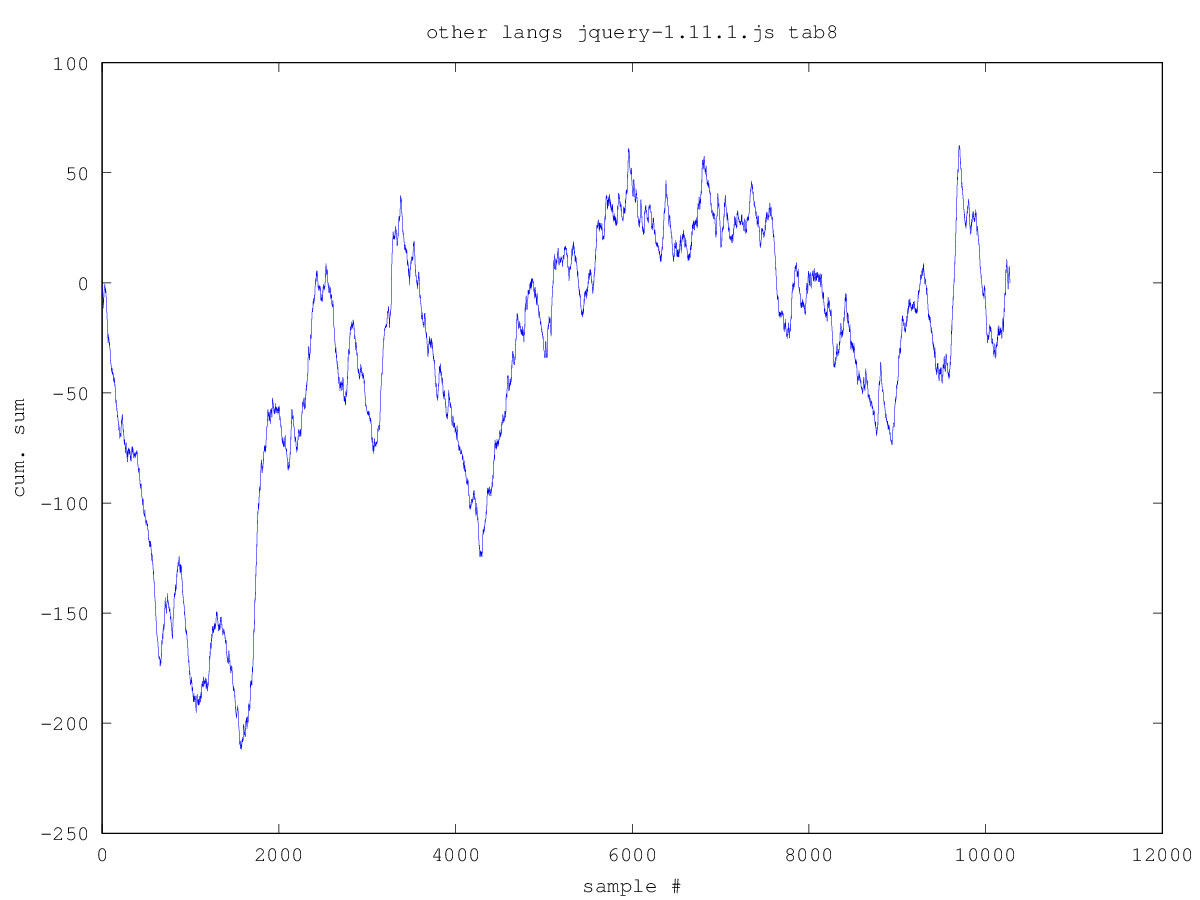
\includegraphics[width=0.8\linewidth]{{fractals/other_lang_data/other_langs_jquery-1.11.1.js_tab8_time_series}.png}
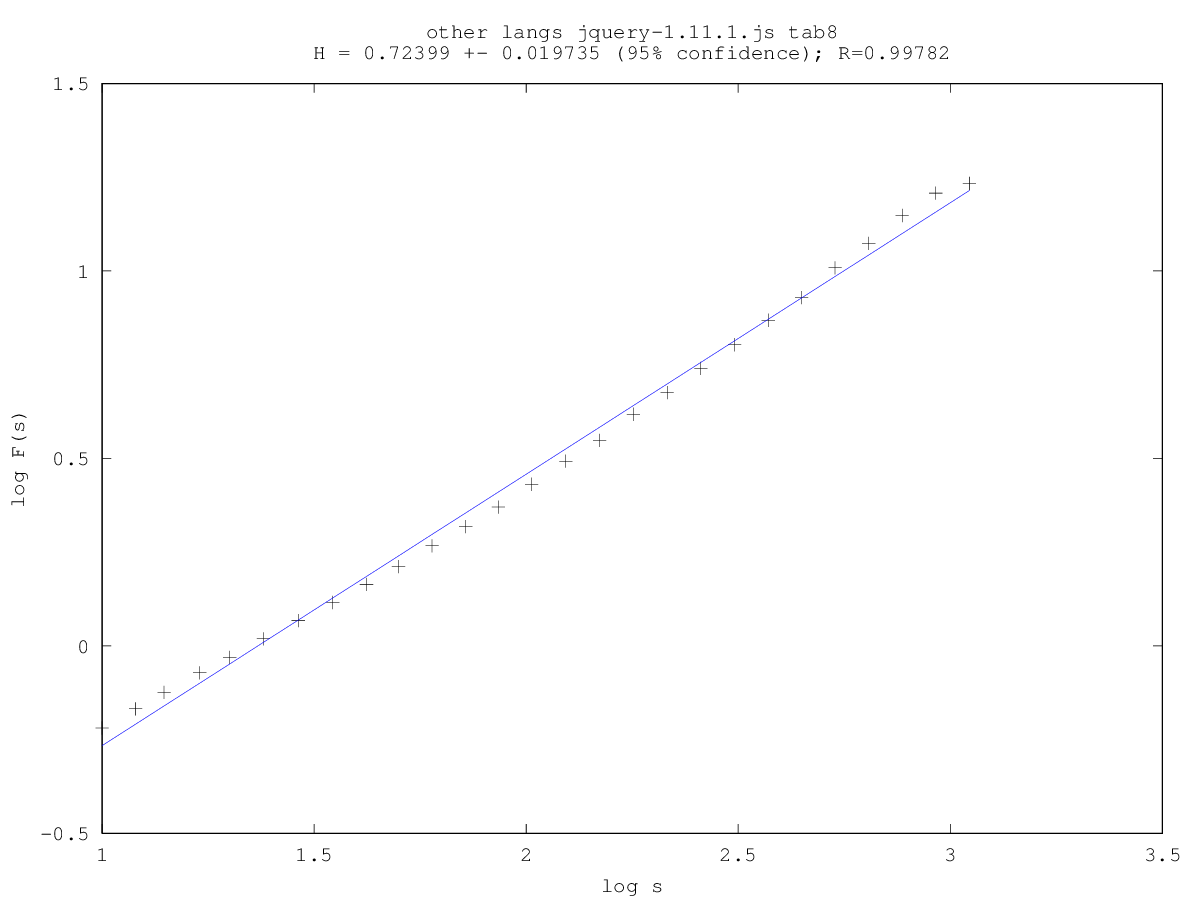
\includegraphics[width=0.8\linewidth]{{fractals/other_lang_data/other_langs_jquery-1.11.1.js_tab8_log_log}.png}
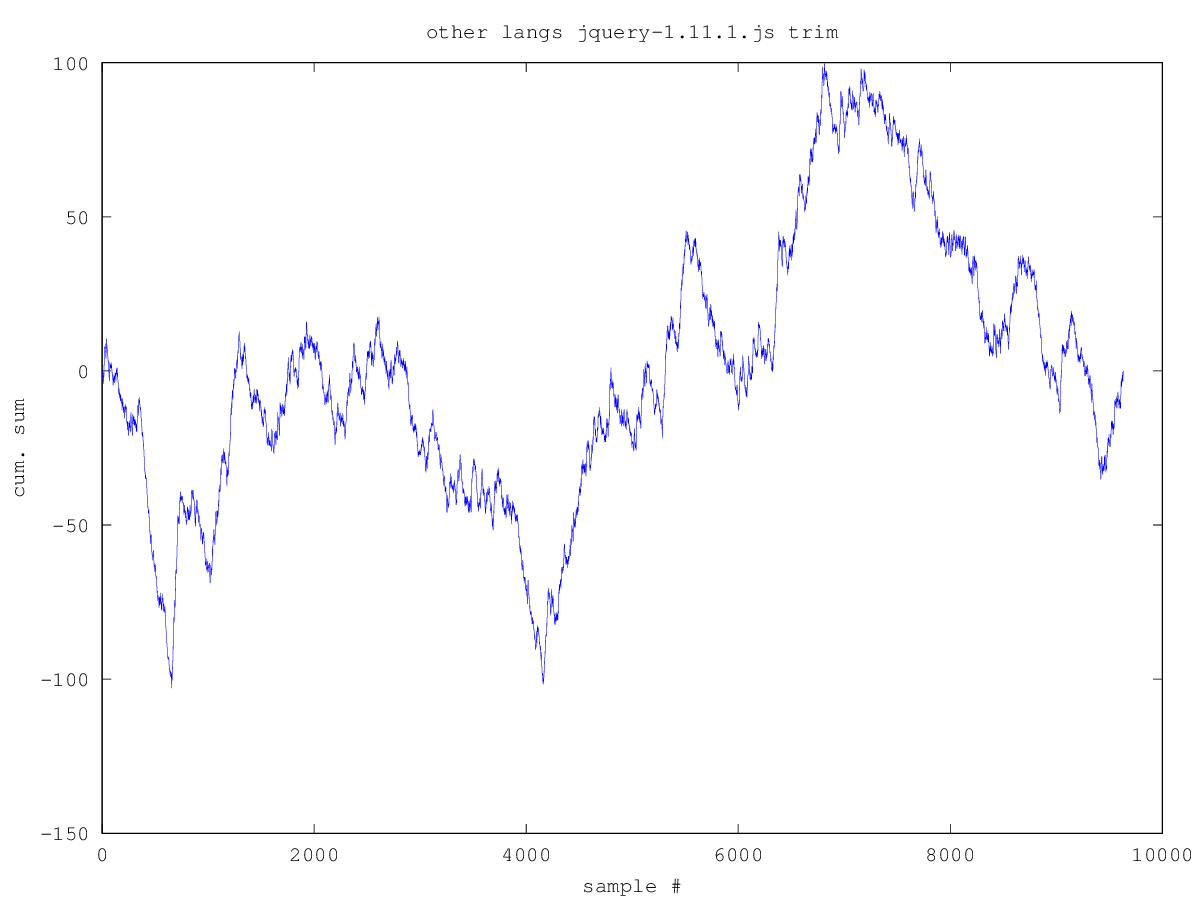
\includegraphics[width=0.8\linewidth]{{fractals/other_lang_data/other_langs_jquery-1.11.1.js_trim_time_series}.png}
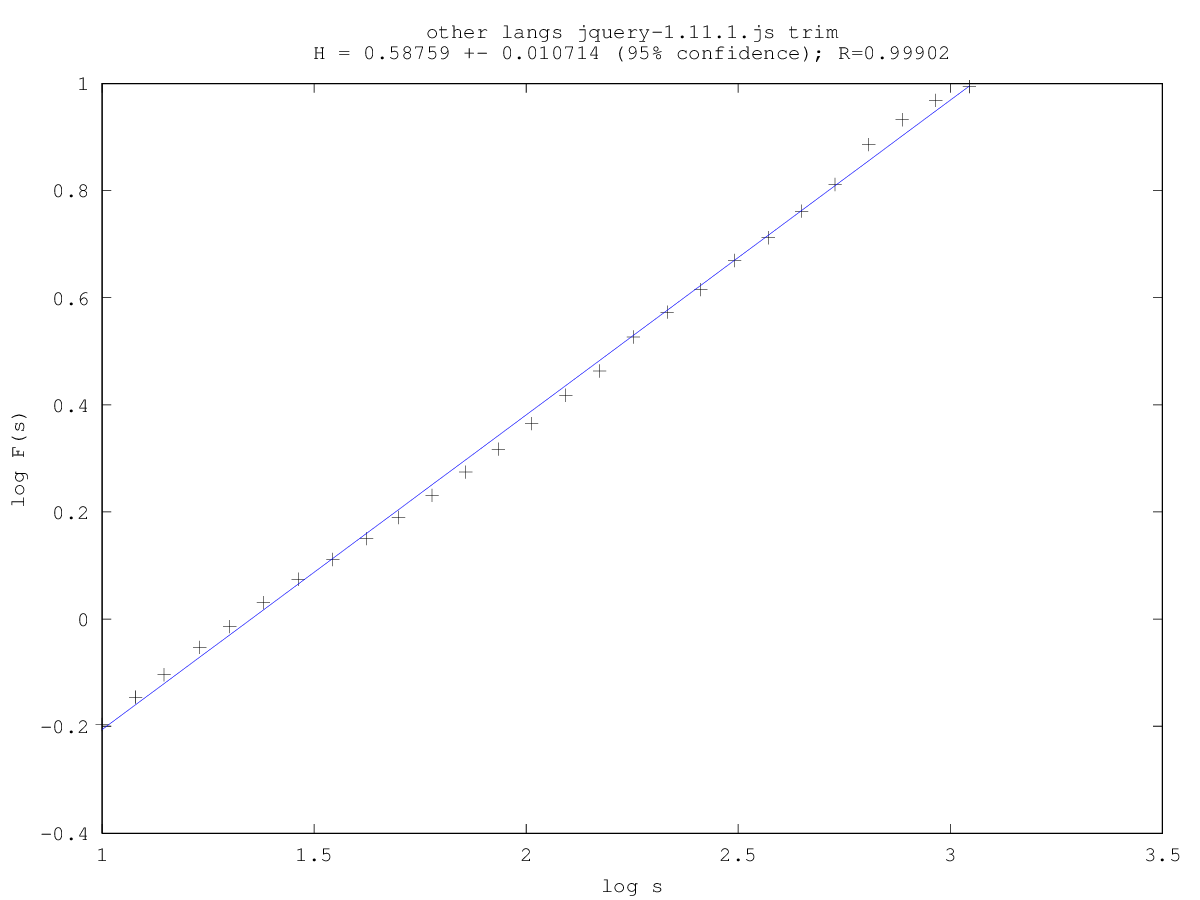
\includegraphics[width=0.8\linewidth]{{fractals/other_lang_data/other_langs_jquery-1.11.1.js_trim_log_log}.png}
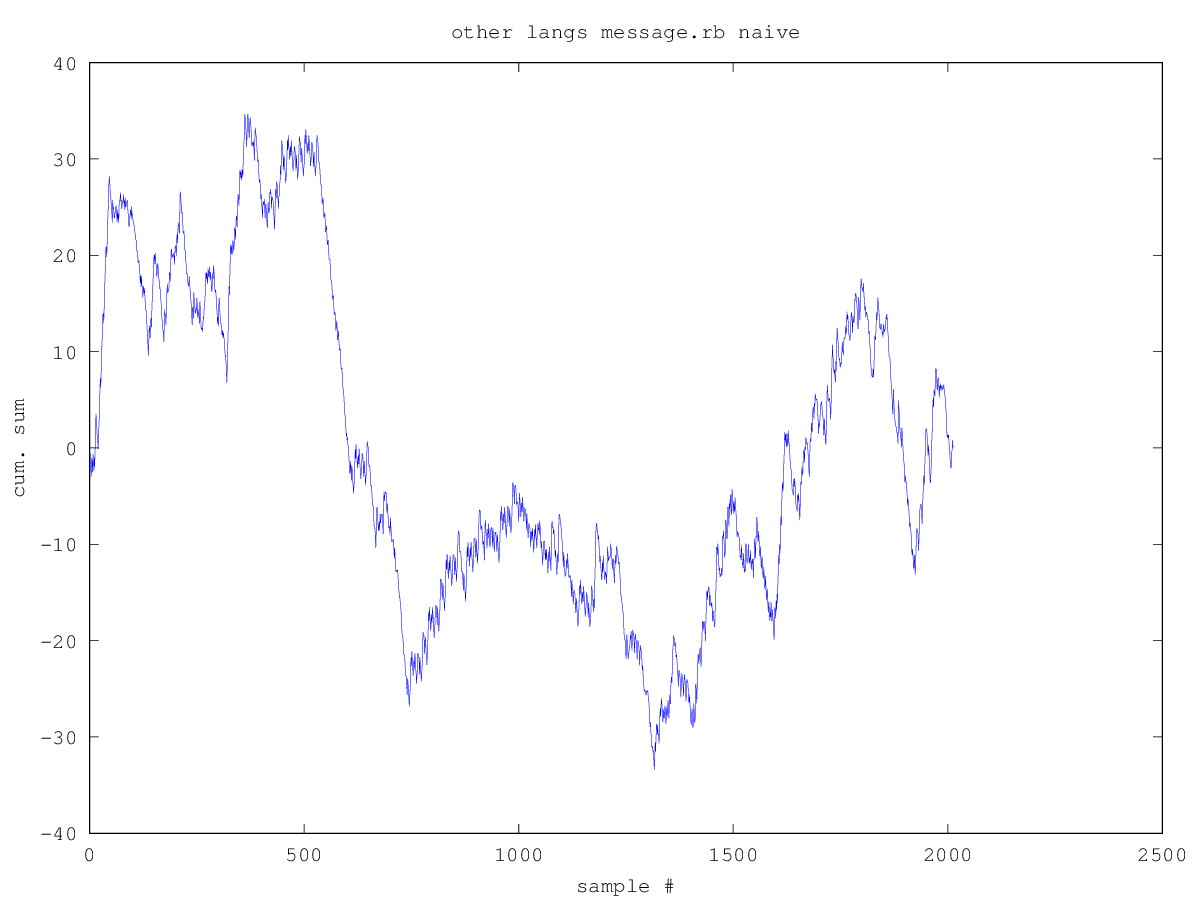
\includegraphics[width=0.8\linewidth]{{fractals/other_lang_data/other_langs_message.rb_naive_time_series}.png}
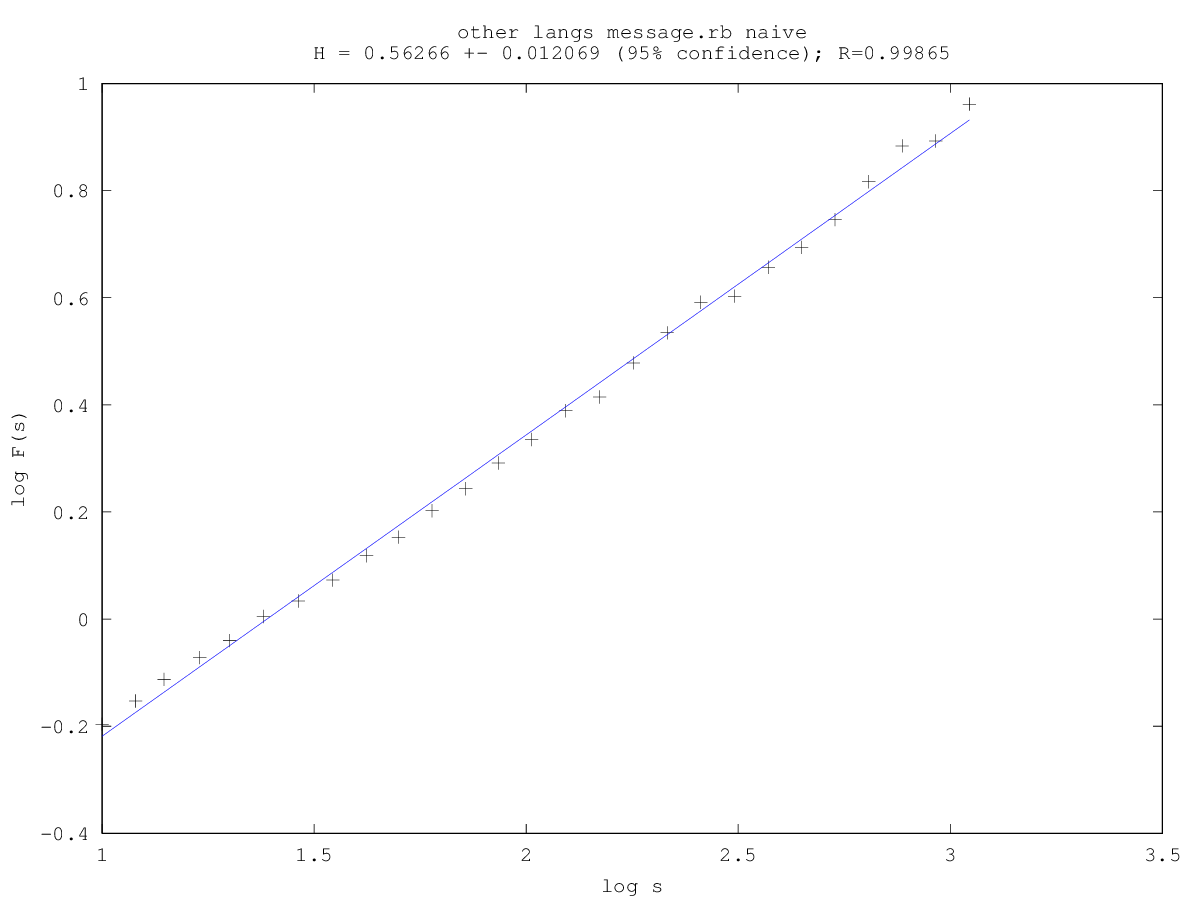
\includegraphics[width=0.8\linewidth]{{fractals/other_lang_data/other_langs_message.rb_naive_log_log}.png}
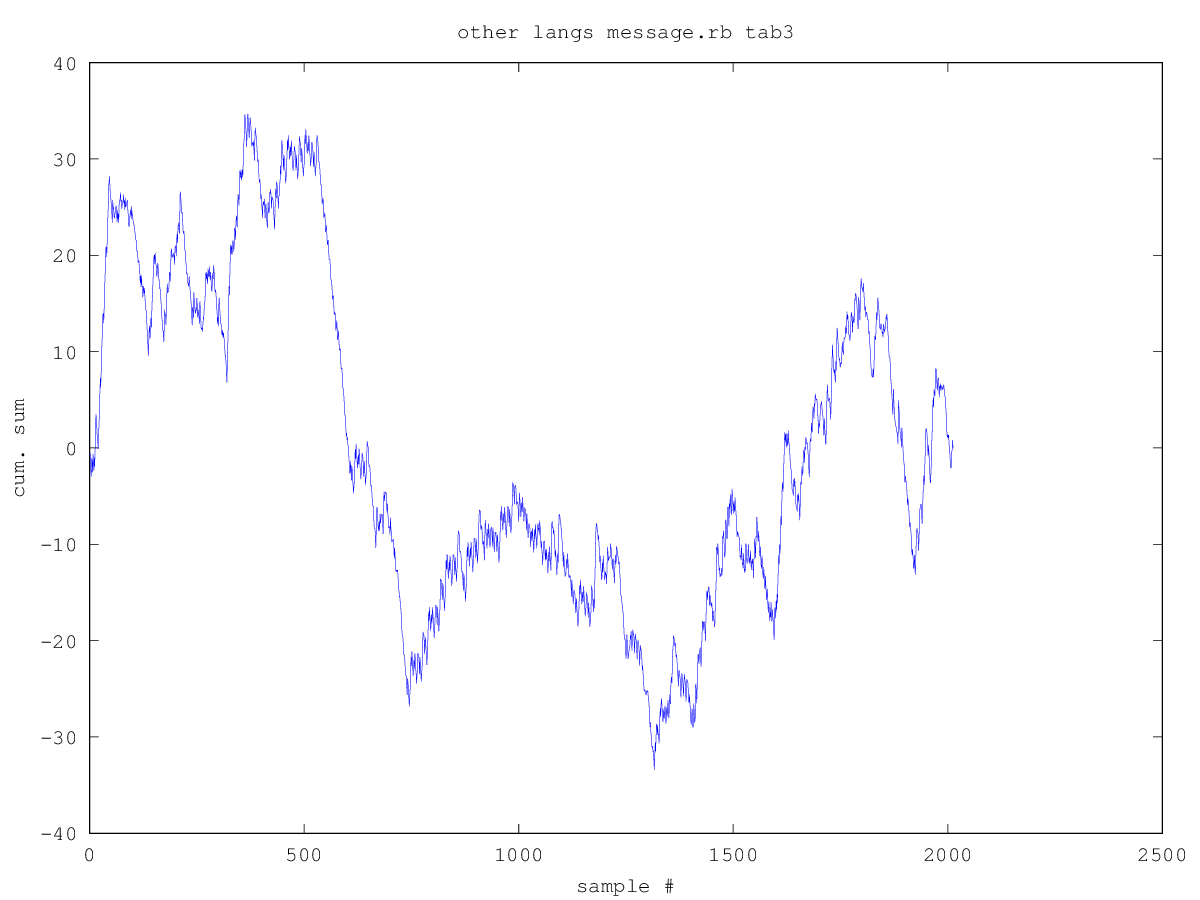
\includegraphics[width=0.8\linewidth]{{fractals/other_lang_data/other_langs_message.rb_tab3_time_series}.png}
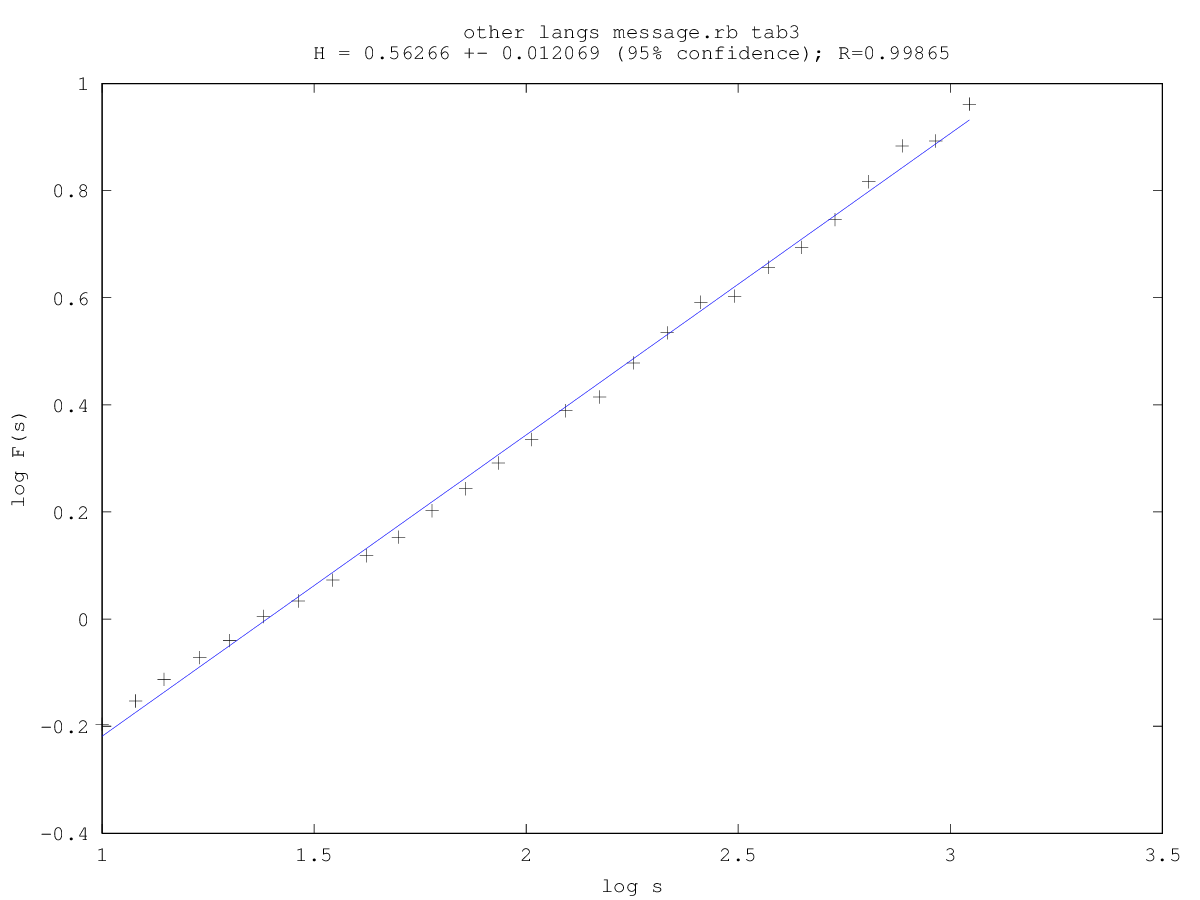
\includegraphics[width=0.8\linewidth]{{fractals/other_lang_data/other_langs_message.rb_tab3_log_log}.png}
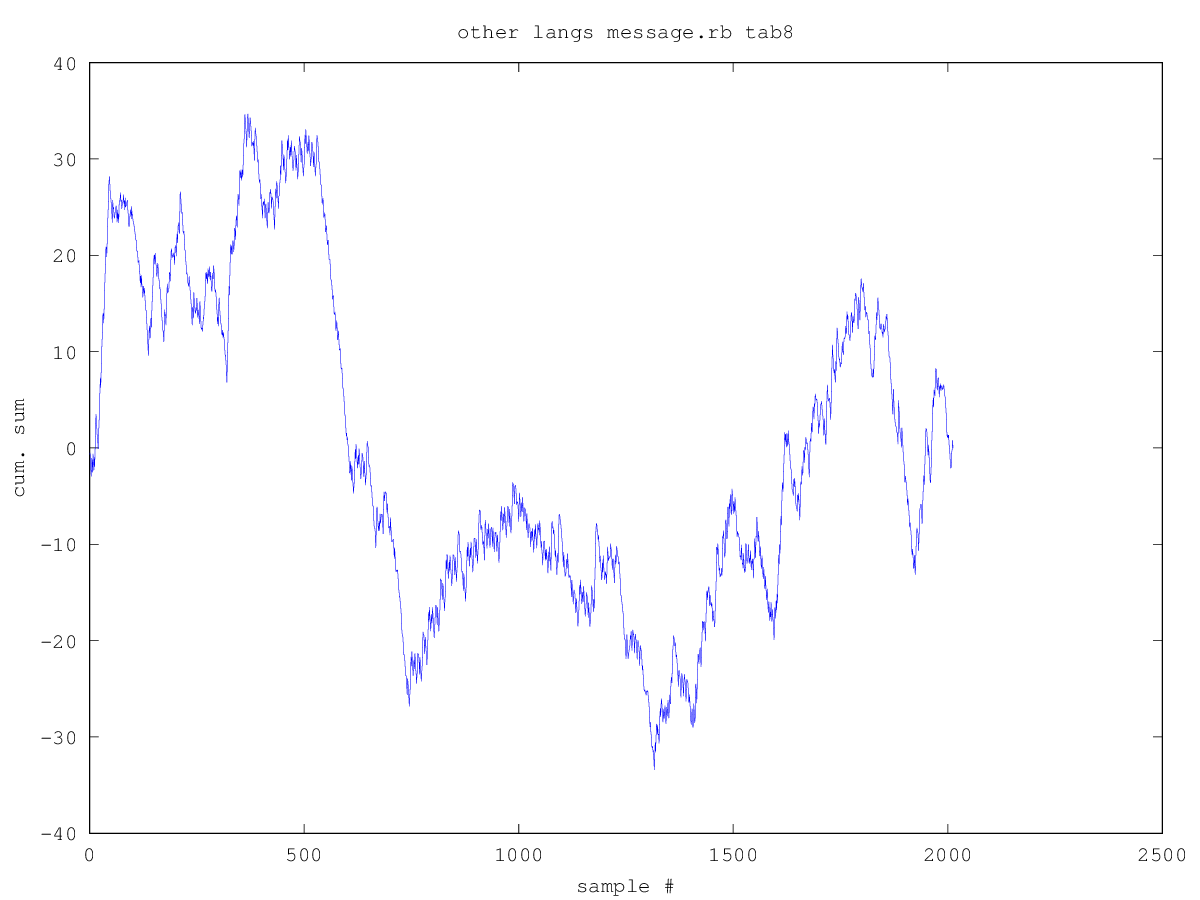
\includegraphics[width=0.8\linewidth]{{fractals/other_lang_data/other_langs_message.rb_tab8_time_series}.png}
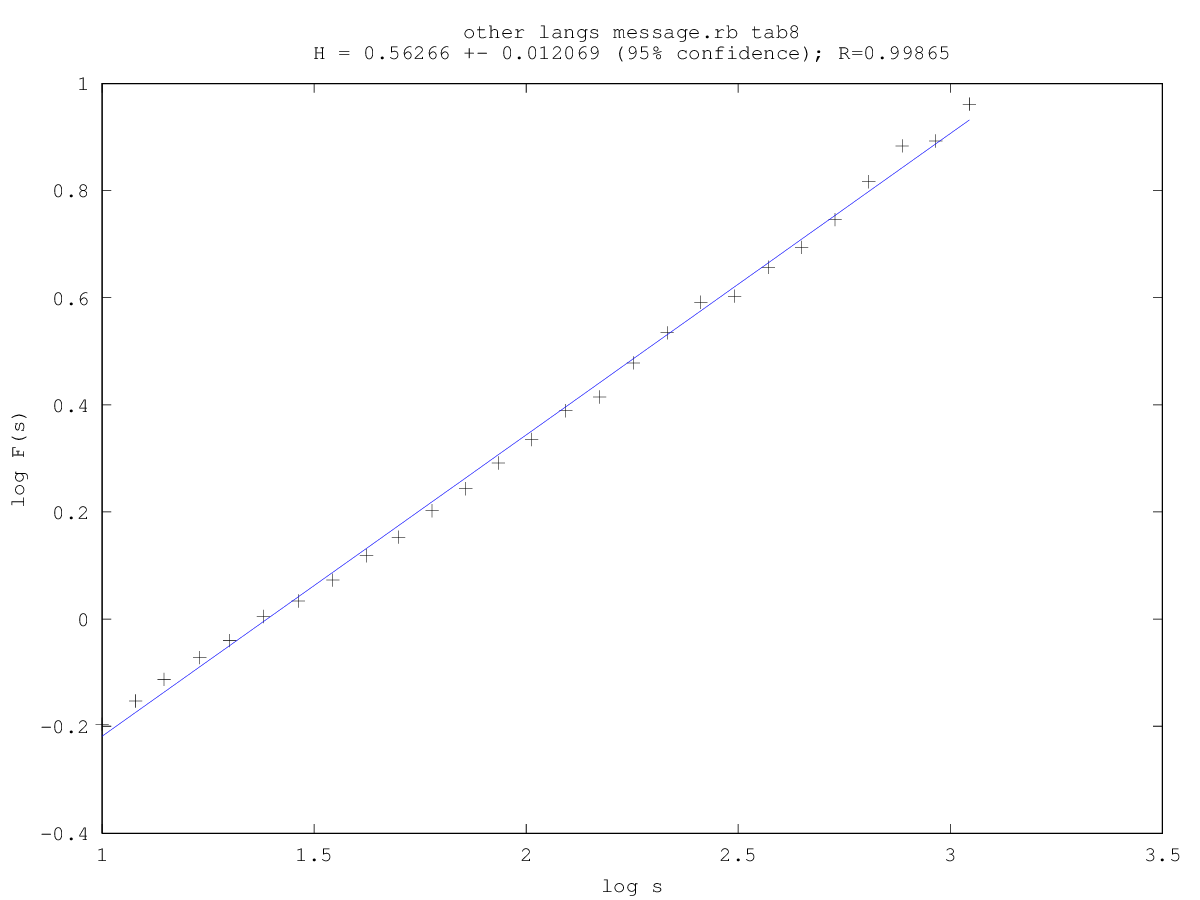
\includegraphics[width=0.8\linewidth]{{fractals/other_lang_data/other_langs_message.rb_tab8_log_log}.png}
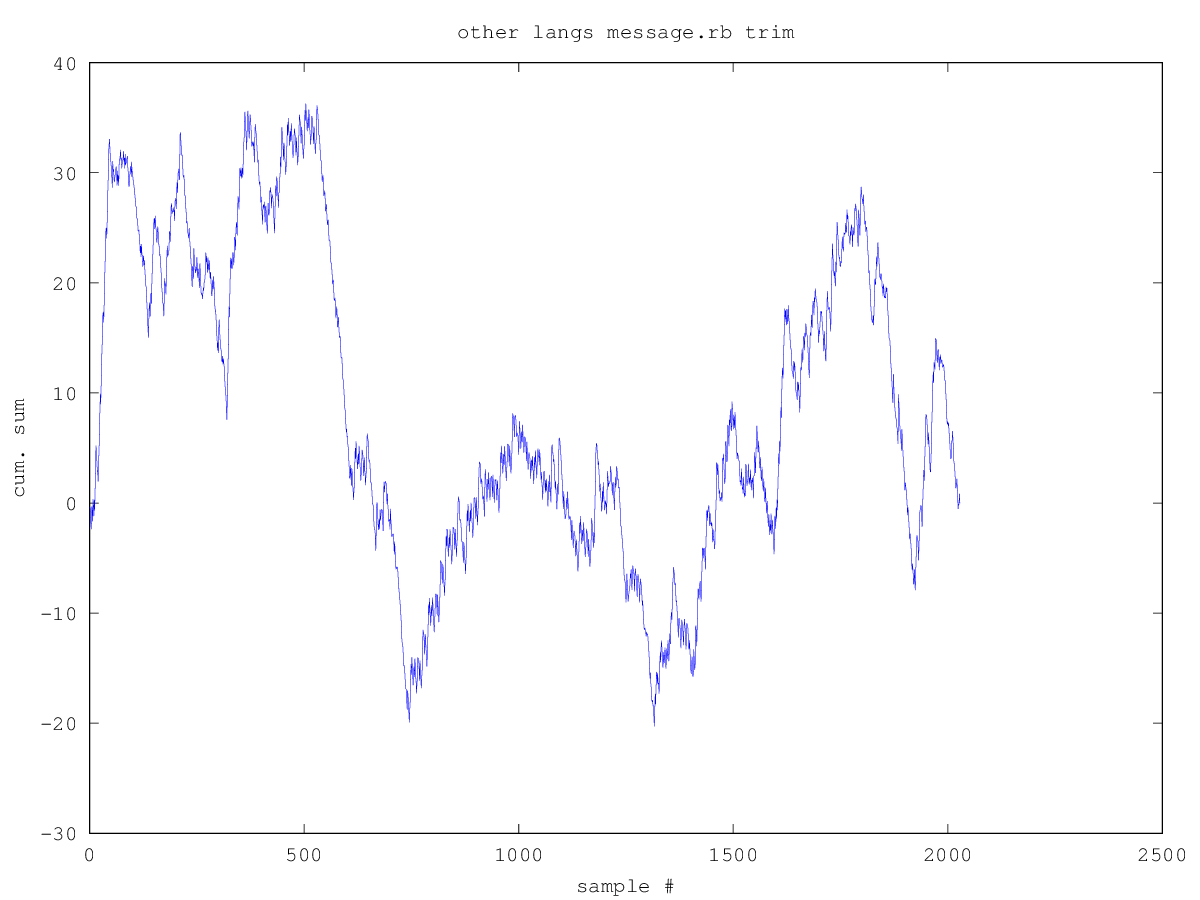
\includegraphics[width=0.8\linewidth]{{fractals/other_lang_data/other_langs_message.rb_trim_time_series}.png}
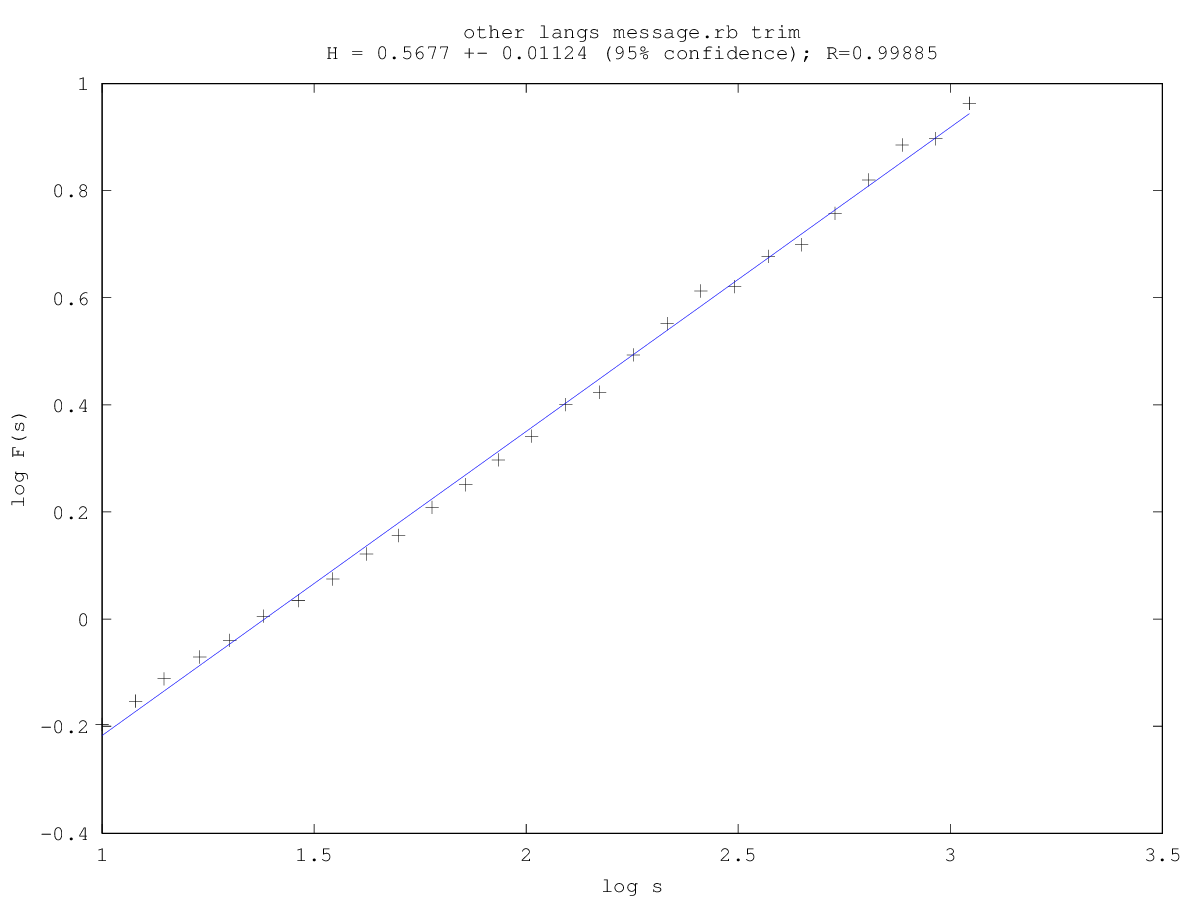
\includegraphics[width=0.8\linewidth]{{fractals/other_lang_data/other_langs_message.rb_trim_log_log}.png}
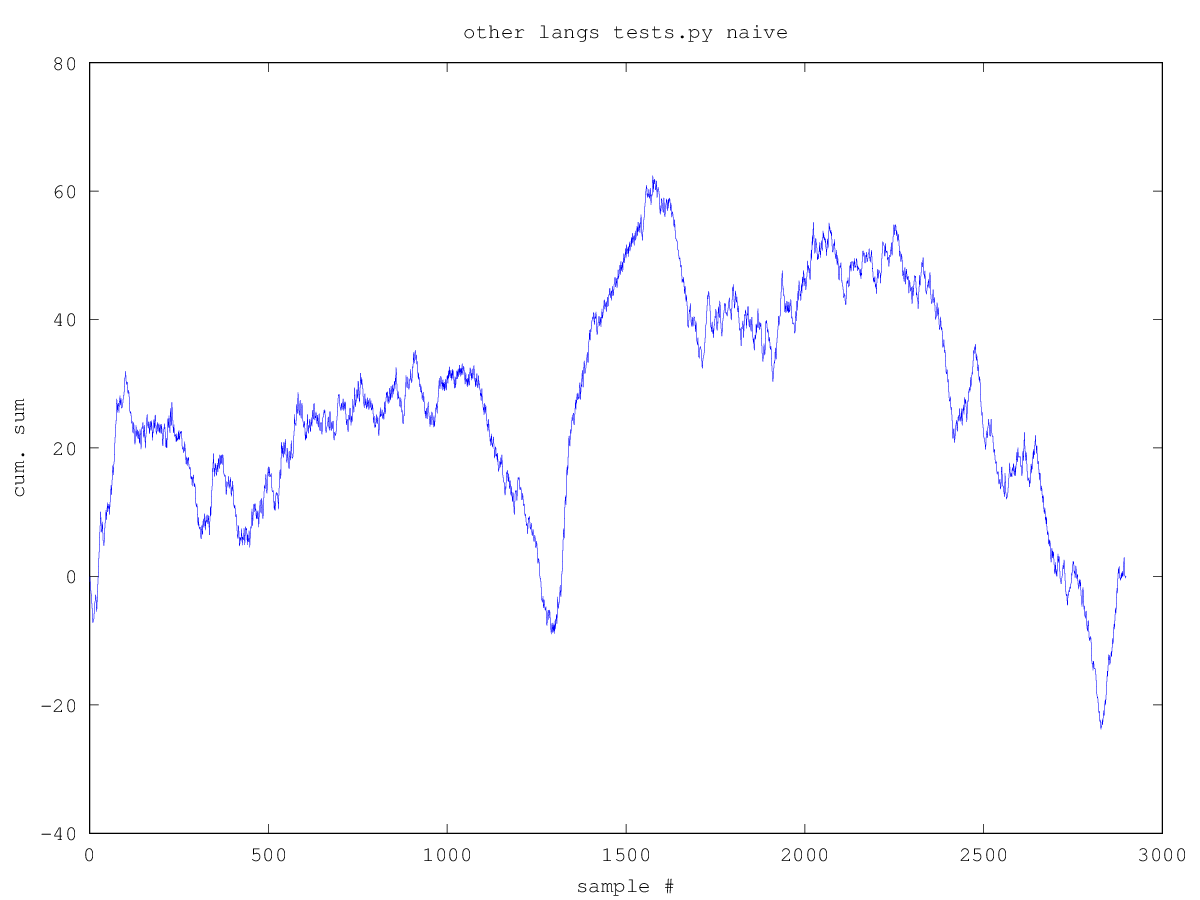
\includegraphics[width=0.8\linewidth]{{fractals/other_lang_data/other_langs_tests.py_naive_time_series}.png}
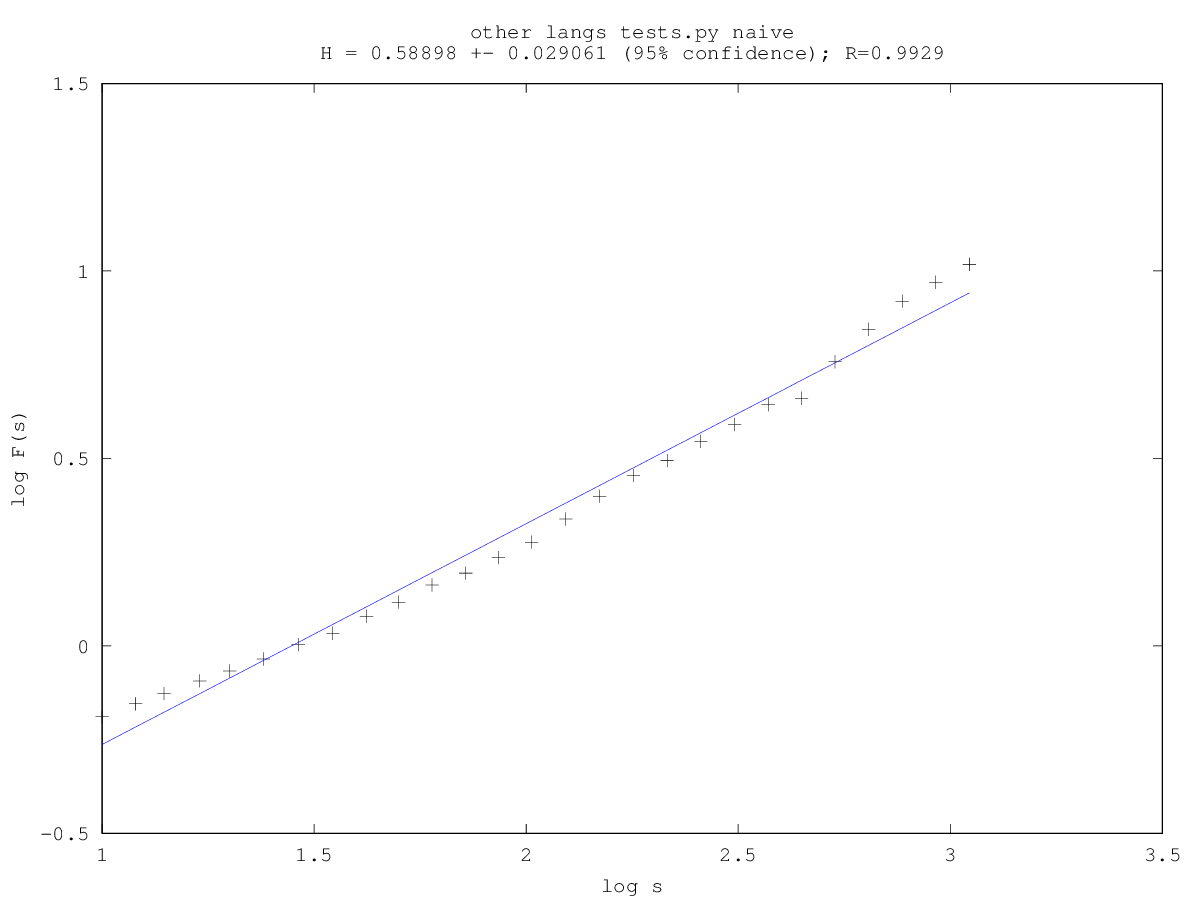
\includegraphics[width=0.8\linewidth]{{fractals/other_lang_data/other_langs_tests.py_naive_log_log}.png}
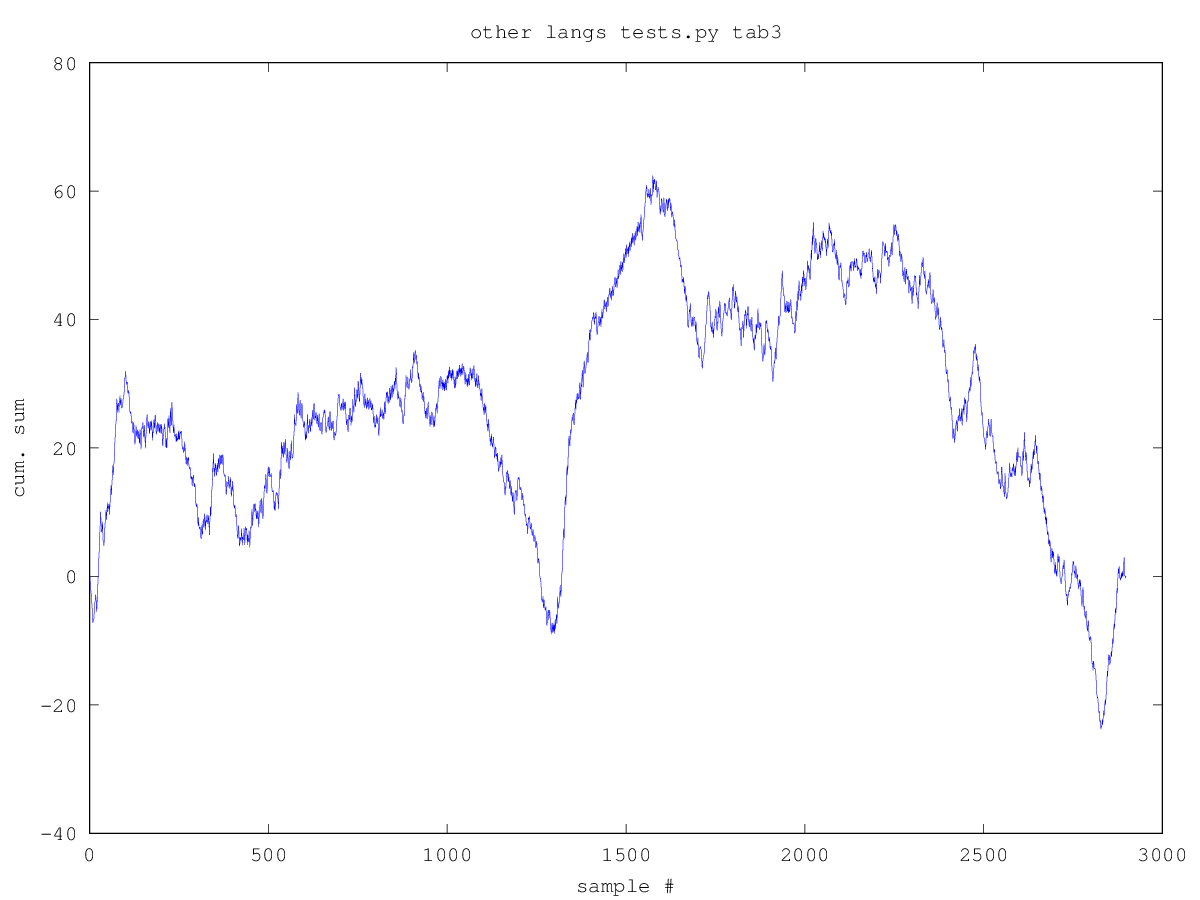
\includegraphics[width=0.8\linewidth]{{fractals/other_lang_data/other_langs_tests.py_tab3_time_series}.png}
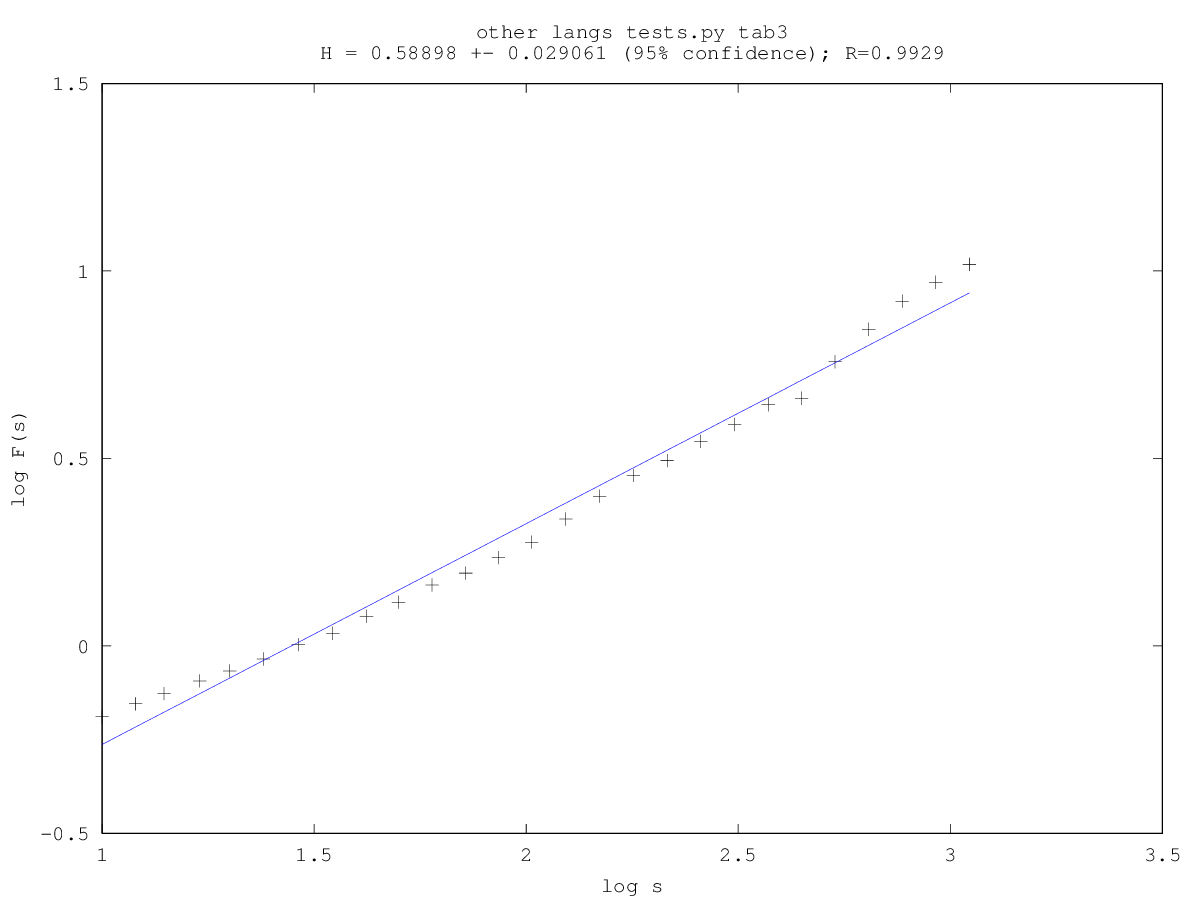
\includegraphics[width=0.8\linewidth]{{fractals/other_lang_data/other_langs_tests.py_tab3_log_log}.png}
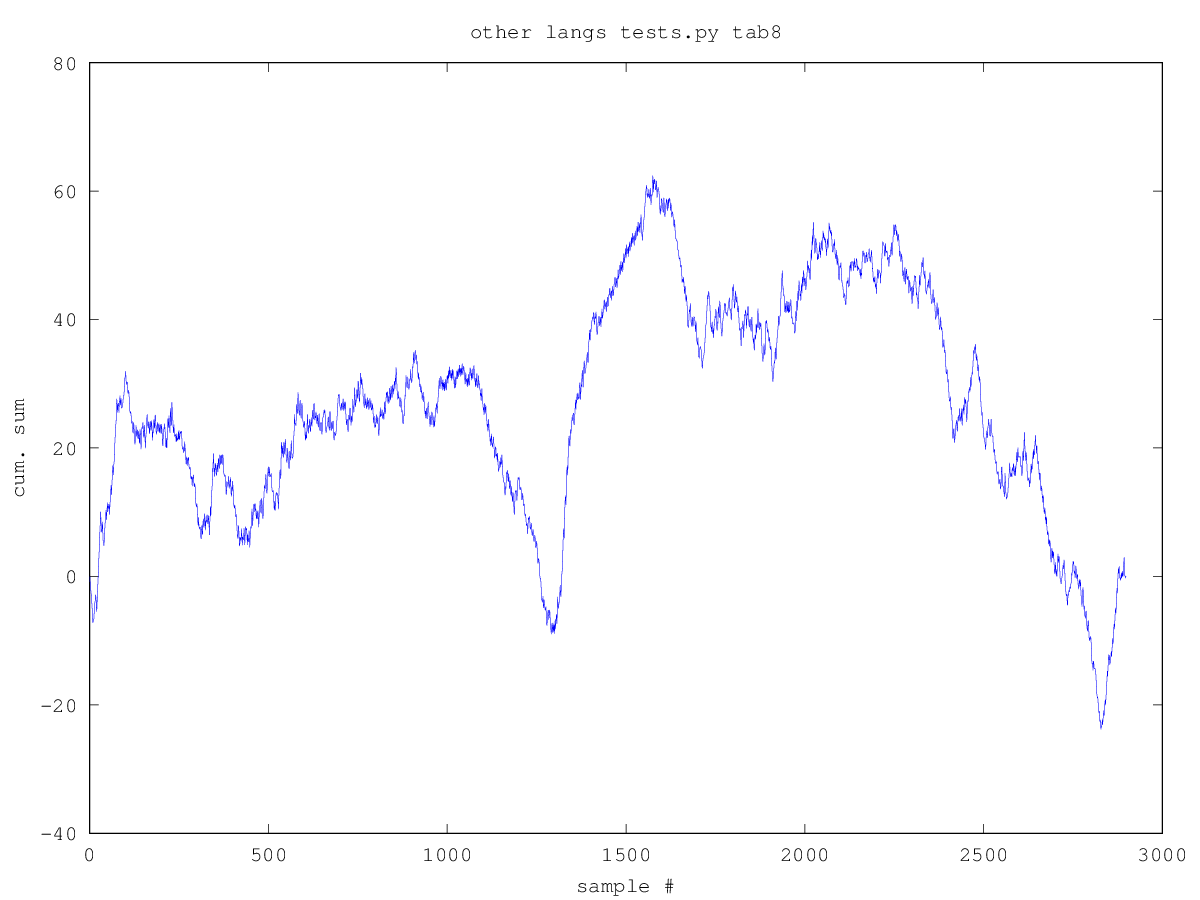
\includegraphics[width=0.8\linewidth]{{fractals/other_lang_data/other_langs_tests.py_tab8_time_series}.png}
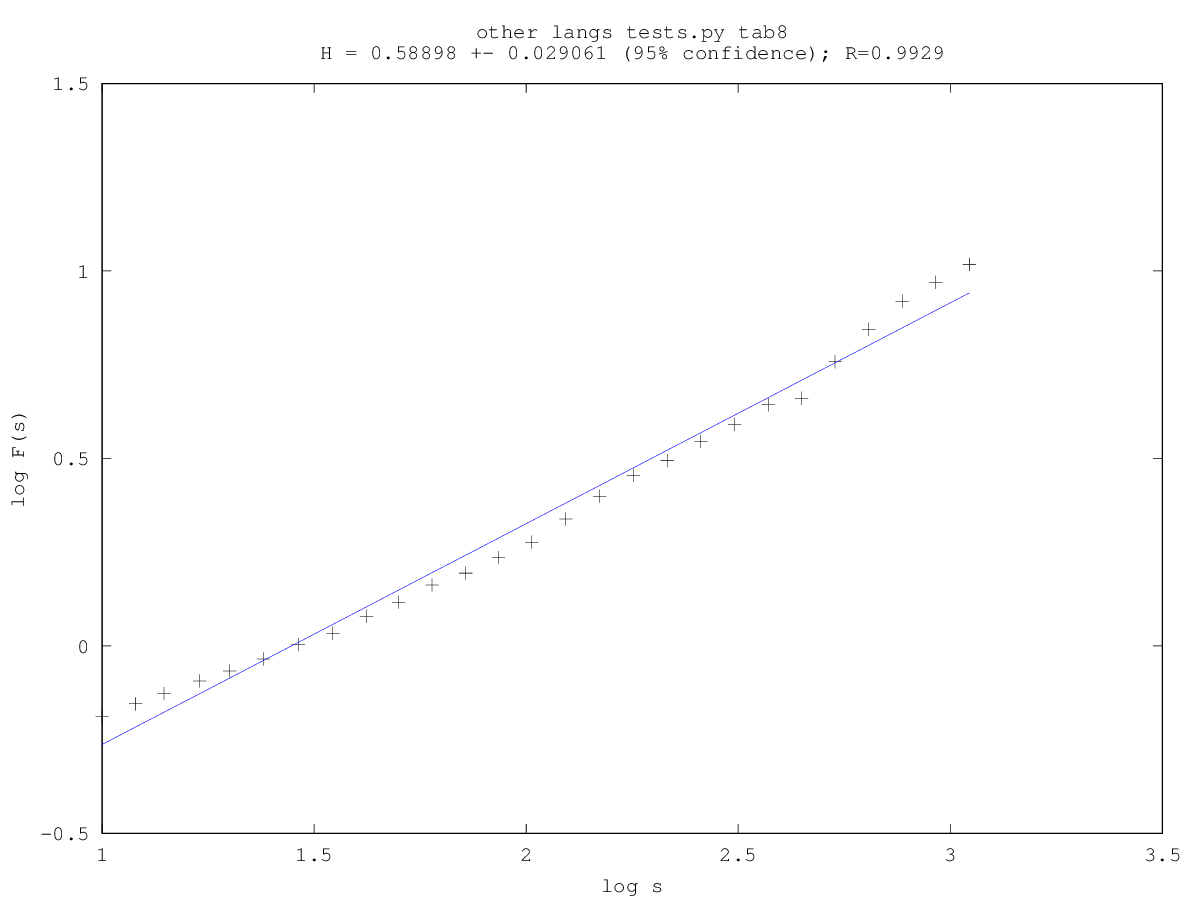
\includegraphics[width=0.8\linewidth]{{fractals/other_lang_data/other_langs_tests.py_tab8_log_log}.png}
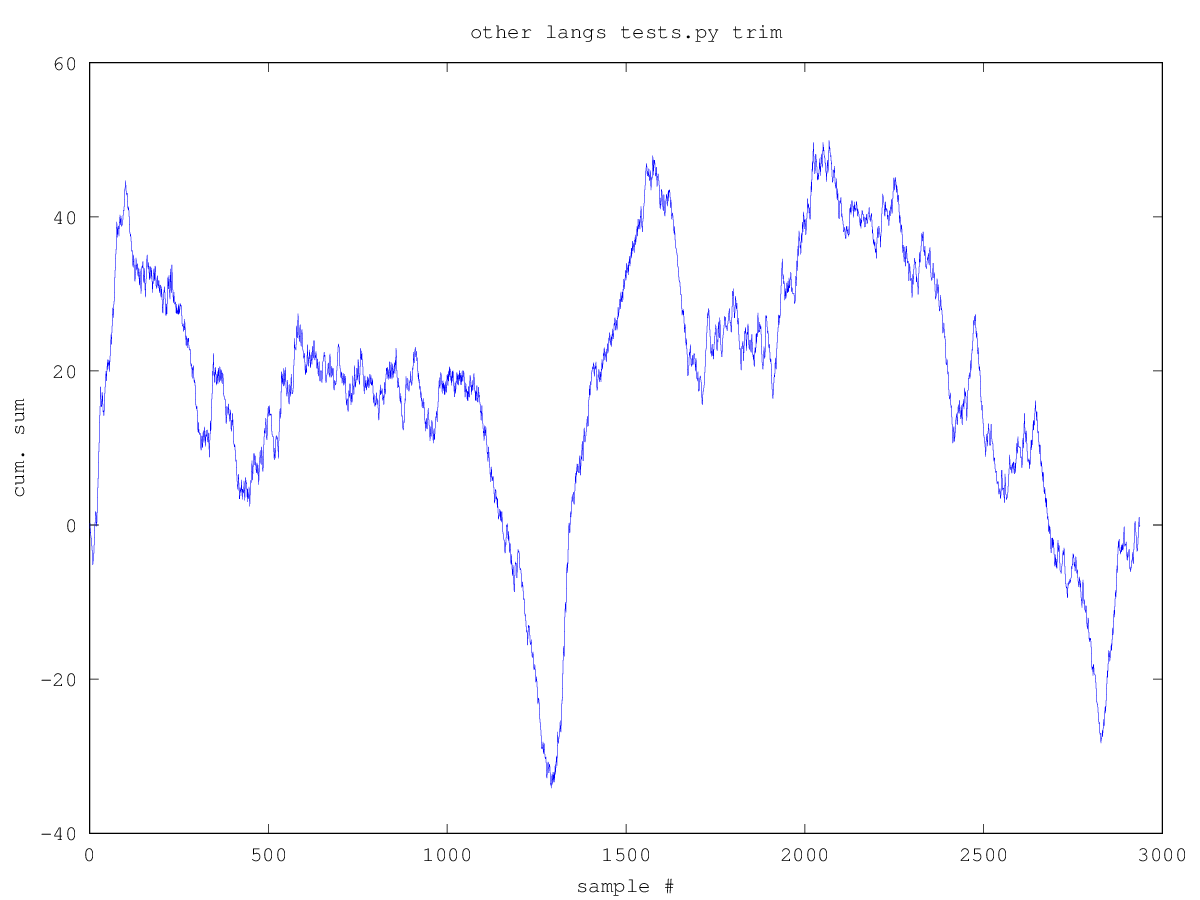
\includegraphics[width=0.8\linewidth]{{fractals/other_lang_data/other_langs_tests.py_trim_time_series}.png}
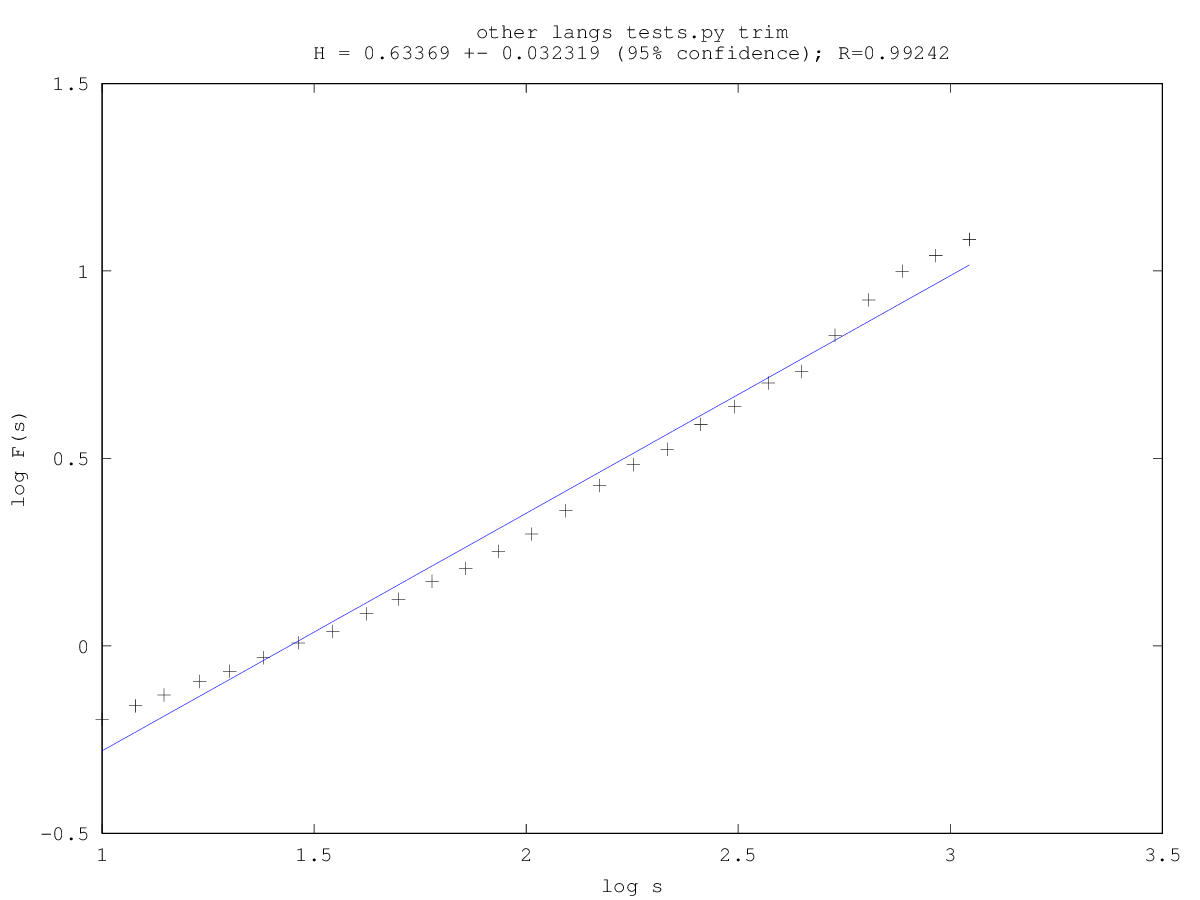
\includegraphics[width=0.8\linewidth]{{fractals/other_lang_data/other_langs_tests.py_trim_log_log}.png}

\end{center}


\end{document}